\documentclass[parskip]{cs4rep}

\usepackage{graphicx}
\usepackage{pseudocode}
\usepackage[T1]{fontenc}
\usepackage{amsmath}
\usepackage{algorithm2e}
\usepackage{array}
\usepackage[labelfont=bf]{caption}
\usepackage{multirow}

\begin{document}

\title{Plan Recognition in Risk}

\author{Jibran A.Z. Khan \& Dr. Michael Rovatsos}

% to choose your degree
% please un-comment just one of the following
%\degree{Artificial Intelligence and Computer Science}
\degree{Artificial Intelligence and Software Engineering}
%\degree{Artificial Intelligence and Mathematics}
%\degree{Artificial Intelligence and Psychology }   
%\degree{Artificial Intelligence with Psychology }   
%\degree{Linguistics and Artificial Intelligence}    
%\degree{Computer Science}
%\degree{Software Engineering}
%\degree{Computer Science and Electronics}    
%\degree{Electronics and Software Engineering}    
%\degree{Computer Science and Management Science}    
%\degree{Computer Science and Mathematics}
%\degree{Computer Science and Physics}  
%\degree{Computer Science and Statistics}    

% to choose your report type
% please un-comment just one of the following
%\project{Undergraduate Dissertation} % CS&E, E&SE, AI&L
%\project{Undergraduate Thesis} % AI%Psy
\project{4th Year Project Report}

\date{\today}

\abstract{
This paper presents the design and implementation of a plan recognition agent for the board game Risk. The agent is based on Geib and Goldman's Probabilistic Hostile Agent Task Tracker (PHATT) algorithm  \cite{Geib:2009:PPR:1550966.1551246}. The agent acts as an observer to the game with the goal of inferring the unknown mission cards based on player actions in real time. We then go on to evaluate the plan prediction accuracy of the agent with four different experiments. The results of these experiments are presented then analysed. We also discuss the project outcomes and propose future work.
}

\maketitle

\newpage

\begin{center}
\textit{I dedicate this dissertation to my mother and father. Without you both; nothing; not a single thing would be possible}
\end{center}

\newpage

\section*{Acknowledgements}

I would like to give a big thanks to Dr. Michael Rovatsos for agreeing to supervise this project. For his herculean efforts in deciphering both my babblings at our weekly meetings and the writings of my cryptic drafts. His involvement has been above and beyond the call of duty. Efcharisto poli!

Thank you to my two little sisters and my family for their unending support in matters both big and small, its always been appreciated. 

A huge thank you to Christopher Geib for taking his time to meet with me, and his attempts to guide a lost undergraduate in the diverse world of plan recognition. His advice in general and his explanations of the PHATT algorithm were invaluable. 

I'd also like to thank Yura Mamyrin and her team at Yura.Net for their work on Domination. In particular Yura who kindly took her time replying to my endless emails.

I want to give a warm thanks to all my friends. In particular, Nick La Rooy for his advice in troubled times and as a constant source of discussion. Punit Bhudia for his encouragement and in helping me collect the data that fuelled this project. To my friends Akash Pandey and Ammar Khan who always been supportive through these four long years. 

Last but not least thank you to all my other friends and acquaintances who participated in my many experiments.

\tableofcontents

%\pagenumbering{arabic}

\chapter{Introduction}

\begin{flushleft}
\textit{AI has the potential to become the new driving force behind computer game innovation.}
\end{flushleft}
\begin{flushleft}
John David Funge, Artificial Intelligence for Computer Games, An Introduction
\end{flushleft}

\section{Motivation}

Artificial Intelligence for games, commonly termed 'game A.I.', has been an area of research since the beginning of significant work in the Artificial Intelligence field. Though techniques for game A.I. have typically come from academia, as John Funge argues \cite{JohnFunge:AIForComp} that academic A.I. and game A.I. are notably different in both scope and application.

Since the primary goal of academia is to further human understanding, often by solving particularly complex problems, the scope of its A.I. techniques are more general in their application.

Game A.I., on the other hand, is built to provide an enjoyable experience for those playing the game, usually by creating the illusion of intelligence. The goal of game A.I. is to control the game environment in a manner that pushes it towards states the game’s designer has chosen. 

Companies in the video game industry who utilise game A.I., which today is the vast majority, tirelessly seek an edge over their competition. This edge has typically come from computer graphics, effects such as hardware shader techniques and the move from two to three dimensional worlds has kept their customers’ interest over the years. 

Emerging though is the idea that as users become accustomed to high quality graphics, developers will require something new to distinguish their product. This will likely be better quality game A.I. And indeed there have already been examples of successful games acclaimed for their game A.I, one such example is F.E.A.R. 

A First-Person-Shooter psychological horror video game, F.E.A.R utilises a S.T.R.I.P.S. style planning-architecture, which developer Jeff Orkin termed Goal-Oriented Action Planning \cite{citeulike:5386647}. The game gained critical acclaim and is commonly referenced as an example of excellent game A.I.

With this shift in focus, there are growing incentives for developers to create more sophisticated game A.I. As in the past, this will likely using techniques from academia. Plan recognition may provide such an opportunity for development.  

Plan recognition is the problem of inferring an agent's plans from observed actions. Significant research in plan recognition began in the 1980's, the results of which have had numerous applications in several fields. Nate Blaylock highlights \cite{oai:CiteSeerPSU:538953} a few of the most prominent as being:

\begin{tabular}{|l|p{8cm}|}
\hline 
\textbf{Field} & \textbf{Some Applications} \\ 
\hline 
User Modelling & Operating Systems, Intelligent Help Systems, Intelligent Tutoring \\ 
\hline 
Multi Agent Interaction & Military Tactical Defence, Multi Agent Coordination \\ 
\hline 
Natural Language Processing & Story Understanding, Machine Translation, Dialogue Systems \\ 
\hline
\end{tabular} 

Plan recognition provides the ability to give highly personalized responses and identify threats from malicious agents. As such, plan recognition algorithms continue to receive attention from various Computer Science communities. 

In video games, plan recognition has been used to perform dynamic analysis in game environments such as Real Time Strategy \cite{conf/aiide/SynnaeveB11} and Multi-User Dungeons \cite{Albrecht:1998:BMK:598277.598308}. More exciting though is the prospect of combining plan recognition algorithms with planning-architectures such as G.O.A.P. or using machine learning to further augment A.I. The desired result is more sophisticated A.I. that is capable of recognising plans and altering its behaviour accordingly. 

\section{Artificial Intelligence and Board Games}

In 1950 Alan Turing published the landmark paper "Computing Machinery and Intelligence", establishing the Turing test, marking what many consider to be the birth of the Artificial Intelligence field. Soon after John McCarthy officially coined the term Artificial Intelligence at a conference in Dartmouth College. He defined it as "the science and engineering of making intelligent machines" \cite{mccarthai}.

Interestingly though, it was thirty five years earlier that Leonardo Torres y Quevedo built "El Ajedrecista", a chess automaton capable of playing a king and rook endgame against a king from any position. Considered the world's first computer game, it was arguably the beginning of Artificial Intelligence and board games, a relationship older than the term Artificial Intelligence itself.  

Since then the relationship has only flourished. Many games such as chess, checkers and backgammon have all been the subjects of research. Each area has seen its various triumphs such as, Chess Grand Master Garry Kasparovs defeat to IBM's chess computer DEEP BLUE in 1997 \cite{aaai/1997w6} and a solution to the game checkers by Jonathan Schaeffer et al in 2007 \cite{SchaefferBBK0LLS05} .

It is clear that the development of A.I. and its application to the medium of games has been, and continues to be, a significant area of interest for both commercial and academic fields. Games are considered a good metric for testing the quality of an A.I. due to their potential for challenging game environments and opponents.

Risk has been the subject of academic work before, with designs for A.I players being a particular focus. In his PhD thesis \cite{michaelwolf}, Michael Wolf of the University of Darmstadt proved that the state space for Risk is infinite. Other research on Risk includes work by students at Stanford University on A.I. players \cite{jlozanodbratz}. They summarise Risk as an interesting opportunity for research, sitting at the "intersection between traditional and modern board games".

\section{Aims}

\begin{itemize}
\item
To design and implement a plan recognition agent for the board game Risk using the PHATT algorithm.
\item
For the plan recognition agent to have an average plan prediction accuracy at least twice that of a uniform guess.
\item
To gain further understanding in the complexities of performing plan recognition in Risk
\item
To determine whether plan recognition algorithms are beneficial in board games, using Risk as an example.
\end{itemize}

\section{Hypotheses}

The hypothesis for the project is that \textit{plan recognition algorithms are beneficial in the board game Risk.}

Beneficial is defined as a combination of two factors. That the plan prediction accuracy is high and the convergence to the correct explanation is fast.

\section{Paper Structure}

Chapter 2 presents a background to the project where the process of plan recognition and the board game Risk are introduced. Reasons for using plan recognition in board games are discussed.

Chapter 3 documents the design of the plan recognition agent. It includes an introduction to the PHATT algorithm, along with a worked example. 

Chapter 4 details the implementation of the plan recognition agent. It includes the high level architecture of the code, as well as modifications to the open source project and relevant design concepts.  

Chapter 5 presents an evaluation of the plan recognition agent, including experiments using the agent. Experimental findings are presented here.

Finally, chapter 6 summarises the conclusions of the project. The main insights and outcomes are discussed and future work is detailed.

\chapter{Background}

\section{Previous Work in Plan Recognition}

Many consider one of the earliest major projects on plan recognition to have been in 1978. Having identified plan recognition as a problem in itself, Schmidt et al \cite{journals/ai/SchmidtSG78} conducted experiments to determine whether or not people inferred the plans of other agents. From their results they created a rule based system called BELIEVER, which attempted to capture the process of plan recognition. 

Three years later, Cohen Perrault and Allen identified two different types of plan recognition: \textit{keyhole} and \textit{intended} \cite{Cohen82a}. 

They defined each as follows:

\begin{itemize}
\item
\textit{Keyhole plan recognition} is the recognition of an agent's plan through unobtrusive observation.
\item
\textit{Intended plan recognition} is the recognition of the plan of a cooperative agent who wishes to be understood.
\end{itemize}

In 1986, Kautz and Allen published a paper titled \textit{Generalized Plan Recognition} \cite{conf/aaai/KautzA86} which set the framework of many plan recognition projects that followed. They formed the basis of plan recognition through logic and reasoning. They defined keyhole plan recognition as involving the identification of a set of top-level goals from possible plans, which could be decomposed into related sub-goals and basic actions, thus creating an event hierarchy also known as a \textit{plan library}. 

It was Charniak and Goldman \cite{journals/ai/CharniakG93} who first argued that plan recognition was largely a problem of reasoning under uncertainty and that any system which did not account for uncertainty would be inadequate. They went on to propose a probabilistic, rather than logic based, approach to plan recognition using Bayesian models. Their research continues to be popular in many avenues of research, including its application to games.

For instance, in 1998, Albrecht, Zukerman and Nicholson \cite{Albrecht:1998:BMK:598277.598308} researched keyhole plan recognition using dynamic Bayesian networks to represent features of an adventure game. The results "showed promise" for various domains. Five years later Fagan and Cunningham utilised case-based plan recognition in the classic game Space Invaders \cite{Fagan03case-basedplan}, producing "good prediction accuracies in real time".

More recently though Synnaeve and Bessiere \cite{conf/aiide/SynnaeveB11} published a paper on the design and implementation of a plan recognition agent in the Real-Time-Strategy game StarCraft. The result of their work was a plan recognition agent capable of predicting the types of units a player intended to produce, through observations of the buildings that they constructed.

\subsection{An Example of Plan Recognition}

We can introduce common concepts, assumptions and the process of plan recognition with an example of an agent attempting to infer the plan of another in a non-adversarial environment. 

Person A is preparing a meal for Person B. For this meal, A can cook just one of two things: a meat burger or vegetarian burger (veg burger). In other words, A has two possible states they wish to reach, or \textit{root-goals}, either a \textit{Cooked-Veg-Burger} or a \textit{Cooked-Meat-Burger}. 

A wants to surprise B, and so will not tell B what his root-goal is. B wants to know what to expect for lunch. Since B cannot know what A is thinking, B must infer A's root-goal through \textit{observing} A cook. In this way, B can consider A's behavioural processes as a Hidden Markov Model. Person B thus models A's behaviour in the following manner. 

Person B assumes that A is rational, and that A has a \textit{plan} to achieve their root-goal. A's root-goal can be decomposed into a number of \textit{sub-goals}, such as \textit{Cooked-Beef-Patties}. Sub-goals can often be decomposed further into \textit{actions} to achieve them, such as \textit{Take-Beef-Patties-Out-Of-Packet}. An important point to note is that these actions are not limited to only being a component of a sub-goal. 

To simplify the example, we introduce the following assumptions:

\begin{itemize}
\item
A believes that they can cook a meal, i.e that their goal is achievable. 
\item
B can only infer the cooking plan of A by observing what A is cooking.
\item
B knows everything that A can cook. 
\item
Through observing A cook, B can predict with certainty what A will cook. 
\item
A cannot hide any actions.
\item
A only wishes to cook one meal.
\item
A has no preferences of what to cook. In other words, given a choice the probability of choosing is equally likely. 
\item
A does not change cooking plan.
\end{itemize}

Given these assumptions and B's knowledge of A's cooking abilities, we can model the set of all of A's plans following the notation set by Geib and Goldman in their paper presenting PHATT.

\begin{figure}[h]
\centerline{
	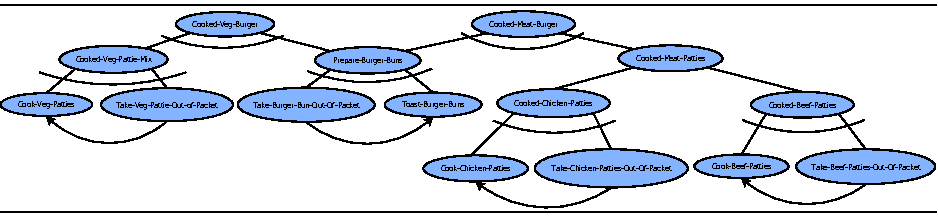
\includegraphics{images/example-plan-library.pdf}
}
\caption{Root-goals are nodes that have no parent nodes. Sub-goals are nodes that have both a parent and children and actions are nodes that have no children. And-nodes are represented by an undirected arc across the lines connecting the parent node to its children. Or-nodes do not have this arc. Actions or goals that are dependant on a previous action are represented by an arc with an arrow.}
\label{fig:example-plan-library}
\end{figure}

To elaborate on the above diagram, one of A's top level or root-goals is \textit{Cooked-Veg-Burgers}. It is an And-node and so accomplishing it requires accomplishing all of its child nodes. 

Children of Or-nodes such as \textit{Cooked-Meat-Patties}, represent choices available to A to accomplish the root-goal. For example to achieve \textit{Cook-Meat-Patties}, A could either accomplish \textit{Cooked-Chicken-Patties} or \textit{Cooked-Beef-Patties}.

Arrows represent dependencies between nodes. For instance to be able to accomplish the action \textit{Cook-Beef-Patties}, A must first perform the action \textit{Take-Beef-Patties-Out-Of-Packet}.

Beginning the example, A first performs the action \textit{Take-Burger-Bun-Out-Of-Packet}, then proceeds to \textit{Toast-Burger-Buns}. At this point, looking at the plan library we have two possible \textit{explanations} for A's behaviour: \textit{Cooked-Veg-Burger} or \textit{Cooked-Meat-Burger}. Each of these explanations are equally likely at this point because the actions that have occurred, so far could be part of either plan.

A then performs the action \textit{Take-Chicken-Patties-Out-Of-Packet}, given our assumptions, we can now conclude that A's root-goal is \textit{Cooked-Meat-Burger} and not \textit{Cooked-Veg-Burger}. In this way B has recognised A's plan, thus performing the process of plan recognition.

\newpage

\section{Introduction to Risk}

RISK is a turn-based board game for two to six players. There are many versions, the first of which was released by french film director Albert Lamorisse in 1957 under the title "La Conqu\^ete du Monde". This paper is only concerned with the standard version of Risk, which is an adversarial environment where players vie for control of a fully observable board representing Earth.

\subsection{Equipment}

\begin{figure}[h]
\centering
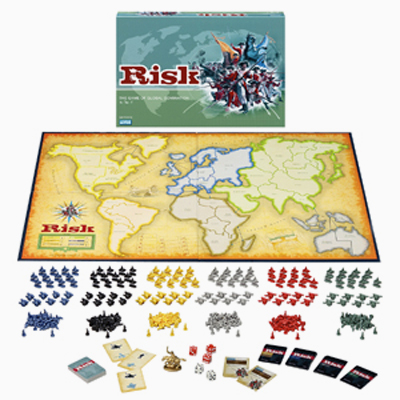
\includegraphics{images/risk-board}
\caption{Risk Equipment \cite{riskimage}}
\label{fig:risk-equipment}
\end{figure}

The game consists of three pieces of equipment:

\begin{itemize}
\item
A board portraying a geographical map of the Earth.
\item
Different coloured tokens called \textit{armies}.
\item
Two fair six-sided dice.
\item
A deck of forty-four cards.
\end{itemize}

\subsection{Rules}

The board is divided into forty two \textit{territories}. Each territory is a partition of the land mass of the Earth. These territories are grouped into six \textit{continents}, usually corresponding to their actual geographic grouping.

Armies are placed on territories. If a player places an army on a territory, this declares that the player \textit{occupies} that territory. Players must have at least one army placed on each territory that they own at all times. Players can choose to place as many additional armies on a territory that they own as they wish.

Each player’s victory conditions depend on the \textit{Game mode}. Game modes significantly impact the behaviour of players and are decided before the game starts. In standard Risk, the possible game modes are:
\newline

\begin{tabular}{|l|p{11cm}|}
\hline 
\textbf{Game Mode} & \textbf{Description} \\ 
\hline 
Domination & Players aim to conquer a certain number of territories, \\ 
\hline 
Mission & Each player is given a single unique mission card. A mission card describes a state they must reach e.g. Occupy North America and Africa, for the rest of the game this is their \textit{root-goal} which only they know. In order to win they can either complete this root-goal or eliminate all other players. \\ 
\hline 
Capital Risk & Each player is given a Capital territory and to win a player must occupy all other Capital territories. \\ 
\hline
\end{tabular} 

This paper is concerned with the mission game mode \textbf{only}. Therefore the following sections only describe the rules for that game mode. 

After the initial setup, each player's turn is split into three distinct phases which always occur in the same order. These phases are:

\begin{enumerate}
\item
Reinforcement
\item
Attack
\item
Movement
\end{enumerate}

In each phase a player performs at least one discrete \textit{action}, which helps to further the players goals, thus forming a sequential task environment.

\subsection{Turn Structure}

\subsubsection{Initial Setup}

The game begins with an initial setup, which involves:

\begin{itemize}
\item
Territories being equally divided between the players with a random allocation.
\item
Players being given a number of starting armies. This number is defined in the Risk rule book. Roughly speaking, it is inversely proportional to the number of players. 
\item
Players distributing their starting armies over their territories.
\item
Each player being given a mission card.
\end{itemize}

\subsubsection{Reinforcement Phase}

At the start of a player's turn, they receive \textit{reinforcements} in the form of additional armies. The act of placing an army in a territory is called \textit{reinforcement}.  The number of additional armies received is based on the number of territories a player occupies and whether they occupy any continents.

\begin{table}[ht]
\centering
\begin{tabular}{|c|c|}
\hline 
\textbf{Occupied Continent} & \textbf{Number of Bonus Armies} \\ 
\hline 
Asia & 7 \\ 
\hline 
North America & 5 \\ 
\hline 
Europe & 5 \\ 
\hline 
Africa & 3 \\
\hline
Australia & 2 \\
\hline
\end{tabular}{}
\caption{Occupied Continent Army Reinforcement Bonus}
\label{table:continent-bonus}
\end{table}

\subsubsection{Attack Phase}

Once a player has distributed their armies from the reinforcement phase, they can choose to \textit{attack}. 

Territories occupied by a player that contain more than one army can attack neighbouring territories occupied by any other player. An attack consists of several \textit{battles}. The outcome of a battle is decided by means of rolling two sets of dice, thus making it a stochastic environment. One set is rolled for the \textit{defender} of the territory and the other for the \textit{attacker}. 

The number of dice each player receives for a battle is dependant on the number of armies placed in each of the players respective territories. The defender receives a die per army up to two armies. The attacker receives a die per army up to three armies not including the single army they are required to have in that territory while occupying it. 

The general rules of engagement are: dice rolls by each player are compared on a one-to-one basis in descending order.. The player with the lower value at each comparison loses a single army; if the die are equal in value the attacker loses an army. The number of comparisons per battle are set by the number of dice the defending player has rolled. The attacking player can commence as many battles as they wish during an attack provided they have the requisite armies.

An attack of a territory has three possible outcomes:

\begin{itemize}
\item
A \textit{Failed-Occupation} by the attacker as they have only one army remaining in which case they must retreat and a \textit{Successful-Defence} by the defender who retains the territory.
\item
A \textit{Failed-Occupation} by the attacker as they choose to retreat before having only one army remaining and a \textit{Successful-Defence} by the defender who retains the territory.
\item
A \textit{Successful-Occupation} by the attacker who occupies the territory and a \textit{Failed-Defence} by the defender who has no armies remaining and so loses the territory. The attacking player, leaving at least one army behind, must then move armies from the territory they attacked from into the newly occupied territory.
\end{itemize}

A player can perform any number of attacks from any territory they own during their turn, provided they have more than one army in the territory they choose to attack from.

\subsubsection{Movement Phase}

When the player chooses to end the attacking phase, or they are no longer able to attack, their movement phase begins.

During their movement phase a player may move armies from one territory to a neighbouring territory they own, provided they leave at least one army behind. This action can only be done once per turn in this phase, after which the movement phase is finished.

After the movement phase has been completed, the player’s turn ends and another player’s reinforcement phase begins.
\newpage

\subsection{Cards}

Each territory has a corresponding card. As well as displaying the name of that territory, each card either depicts an infantry, cavalry or artillery symbol. By successfully occupying another player's territory in a turn, a player is awarded a single card for that turn. There are also two wild cards which can be assigned a symbol of the player’s choosing. Owning a set of three cards with the same symbols or a set of three distinct symbols gives the player the opportunity to trade the set of cards for additional armies. This trade can be done at any point during the player’s turn. 

\section{Why Plan Recognition in Board Games}

By "knowing a users plan and goals can significantly improve the effectiveness of an interactive system" \cite{Carberry:2001:TPR:598284.598348}, to this board games are most definitely not exempt. With the success seen in the application of plan recognition to video games, often in complex environments, gives rise to optimism to transferring this success to board games.

"Knowing a user’s plan and goals can significantly improve the effectiveness of an interactive system" \cite{Carberry:2001:TPR:598284.598348}. The successes seen in the application of plan recognition to video games, many of which have highly complex environments, indicates that similar successes can be had with board games. 

Molineaux, Aha and Sukthankar argue that "plan recognition methods can be a powerful ally for machine learning techniques" \cite{Molineaux09g.:beating}. Indeed, this was demonstrated by  Synnaeve and Bessiere’s work with StartCraft \cite{conf/aiide/SynnaeveB11}. Their plan recognition agent utilised unsupervised machine learning of common plans, which could be used as input for adaptive A.I. Using similar techniques for augmenting board game A.I. is an attractive proposition. 

\section{Summary}

Plan recognition is a mature area of research dating back to the 1950's. It has seen applications in a variety of fields including video games. Risk a popular board game that provides an interesting environment to test the application of plan recognition algorithms. It is a multi-agent adversarial environment at the intersection between modern and classical board games. Plan recognition techniques have been used before to augment video game A.I.; there are similar opportunities for applying them to board games. Machine learning can be used to create more interesting A.I. opponents.

\chapter{Design}

\section{Introduction to PHATT}

PHATT is a plan recognition algorithm by Christopher Geib and Robert Goldman \cite{Geib:2009:PPR:1550966.1551246}. PHATT operates on plans that are executed dynamically, but in discrete time steps. The set of actions that an agent can take each step, their \textit{pending set}, depends on the actions that the agent has previously taken.
The model is as follows. An agent first chooses a root-goal, then a set of plans to achieve that root-goal. Any actions of those plans that had no pre-requisite actions would form the initial pending set of the agent. The agent would then perform an action from the initial pending set, which results in some actions being appended to the pending set and others being removed, thus forming the next pending set. Assuming \textit{blind commitment} on the part of the agent, the agent would then continue to perform actions until its root goal has been satisfied.

From this model, Geib and Goldman proposed an algorithm utilizing a Bayesian approach to perform probabilistic plan recognition. 

The algorithm computes \textit{Pr(g}|\textit{obs)} - the conditional probability of a root-goal \textit{g} given a set of observations \textit{obs} - or its equivalent form \textit{Pr(exp}|\textit{obs)}, the conditional probability of a particular explanation \textit{exp} that the agent had a root-goal, given a set of observations \textit{obs}.

Using Bayes’ Rule they defined \textit{Pr(exp}|\textit{obs)} as:\newline

\centerline{
\textit{Pr(exp}|\textit{obs)} = \textit{Pr(exp} $\wedge$ \textit{obs)} / \textit{Pr(obs)}
}

They then (as other practical Bayesian systems do) exploited the equivalent formulae:\newline

\centerline{
\textit{Pr($exp_0$}|\textit{obs)} = \textit{Pr($exp_0$} $\wedge$ \textit{obs)} / $\displaystyle\sum\nolimits_{i}$ \textit{Pr($exp_i$} $\wedge$ \textit{obs)}
}

This is the conditional probability of the explanation $exp_0$ being computed by dividing the conditional probability of $exp_0$  by the sum of the probability mass associated with all possible explanations.

\subsection{Computing an Explanation's Probability}

Computing the term \textit{Pr(exp} $\wedge$ \textit{obs)} requires the plan library to be augmented with three probabilistic features:\newline

\begin{enumerate}
\item
The prior probability of the root-goal.
\item
The respective probabilities of choosing any sub-goals.
\item
The probabilities of picking actions from the agents pending set.
\end{enumerate}

The probability of an explanation is then calculated by multiplying each of the terms together in the following manner: \newline

\centerline{
\textit{Pr(exp} $\wedge$ \textit{obs)} = \textit{Pr}(\textit{goals})\textit{Pr}(\textit{plans}|\textit{goals})\textit{Pr}(\textit{obs}|\textit{exp})
}

\section{Environment Modelling and Data-Structure Design}

PHATT is designed to work in an action space. It was therefore it was a vital to translate Risk into such an action space. 

Solving this issue involved modelling and data structure design. By exploiting the environmental constraints on what a player can do, and observing the choices they made given these constraints, we attempt infer the plan of a player.

\subsection{Root-Goals}

The mission cards of the Risk environment are the root-goals. These are:

\begin{itemize}
\item
Occupy Europe, Australia and one other continent.
\item
Occupy Europe, South America and one other continent.
\item
Occupy North America and Africa.
\item
Occupy North America and Australia.
\item
Occupy Asia and South America.
\item
Occupy Asia and Africa.
\item
Occupy 24 territories.
\item
Occupy 18 territories and occupy each with at least two troops.
\item
Eliminate a player.
\end{itemize}

Since mission cards are handed out at random, the prior probability of a root-goal is 1/$n$, where $n$ is the number of mission cards. The data structure of a root-goal is therefore in the form of a tuple containing the name of the root-goal and its prior probability: 

\centerline{
 $RG = ( rootGoalName, 1/n)$\newline
}

The collection of these data structures form the basis of the term \textit{Pr}(\textit{goals}) in the computation of \textit{Pr(exp} $\wedge$ \textit{obs)}.

A subset of these, where the root-goal involved occupying continents only, were chosen to be the focus of this paper. This choice was made due to time constraints and is an avenue for future work.

Root-goals involving occupying continents can be defined as one of two types:

\begin{enumerate}
\item
\textit{Two-Continent}: Players must occupy two explicitly named continents.
\item
\textit{Two-Continent+1}: Players must occupy two explicitly named continents and another of their choice.
\end{enumerate}

\textit{Two-Continent} are explicit in their sub-goals, but \textit{Two-Continent+1} type root-goals can be decomposed into \textit{children-root-goals}. Children-root-goals of a \textit{parent-root-goal} are a result of a different choice of sub-goals. The number of children-root-goals of a parent-root-goal depends on the environment. For example the root-goal Occupy Europe, South America and one other continent can be expressed as any of the following children-root-goals:

\begin{itemize}
\item
Occupy Europe, South America and Asia.
\item
Occupy Europe, South America and Africa.
\item
Occupy Europe, South America and North America.
\item
Occupy Europe, South America and Australia.\newline
\end{itemize}

Each is a valid root-goal in itself, but are still children of the same parent-root-goal. Therefore, the assumption is made that when the plan recognition agent predicts one of the children-root-goals when the players mission card is the parent-root-goal, it is classified as a correct prediction. A modelling difference followed this assumption. 

By hard coding every root-goal as explanations of a players behaviour; then assigning that full set of explanations to each player from the start of the game, provided that action probabilities are computed, multiplied with each respective explanation, normalised and then stored immediately as soon as the action occurs. Removes the need to store a history of pending sets, to save a list of actions a player has taken or to create and calculate new instances of explanations. This method is similar to that of the 'Test and Generate' algorithm proposed in PHATTs paper rather than the dynamic algorithm proposed at the end of the paper.

This has another implication. Since PHATT computes \textit{Pr(exp} $\wedge$ \textit{obs)} by multiplying three terms together, choosing to operate on a fully enumerated set of root-goals removes the need to compute player choice as we consider every case from the start hence the term \textit{Pr}(\textit{plans}|\textit{goals}) is equal to one for all explanations.

What is then measured over the course of the game is the probability of each explanation of a player’s behaviour, and the highest probability by the end of the game is the plan recognition agent’s prediction.

\subsection{Actions}

In Risk the only actions players perform are:

\begin{itemize}
\item
Attacking Territories.
\item
Defending Territories.
\item
Occupying a Territory.
\item
Reinforcing Territories.
\item
Moving armies.
\item
Trading Territory Cards.
\end{itemize}

Each of these action must be modelled in a manner that contributes towards an explanation of a player's behaviour.

\subsubsection{Attacking}

Though players can perform several attacks during their turn, they can only attack one territory at a time. Thus, players must choose both which territories to attack and the order in which to attack them, provided they have neighbouring territories and sufficient armies. Modelling these choices provides an avenue to infer a player’s plan.

The pending set of a player's attack actions for any given turn is the aggregate of either a successful or unsuccessful attack on each territory that the game rules will allow them to attack. 

If a player $p$ successfully occupies a territory $T_{o}$, then the attack actions of neighbouring territories of $T_{o}$ are added to $p$'s attack pending set. If they lose a territory $T_{l}$ due to another player's successful attack, then any attack actions of neighbouring territories of $T_{l}$ are removed from their attack pending set for their next turn. 

The attack action is a singular event that is either \textit{consistent} or \textit{inconsistent} with explanations of a player’s behaviour. 

For example, given three explanations:

\begin{enumerate}
\item
Occupy North America and Australia.
\item
Occupy North America and Africa.
\item
Occupy Asia and South America.
\end{enumerate}

Successfully occupying a territory in North America would be \textit{consistent} with explanations 1 and 2, but \textit{inconsistent} with 3. In probabilistic terms, the likelihood of 1 and 2 would rise whereas 3 would fall.

Having defined the outcome of attacks as either successful or unsuccessful, attacks can be decomposed into the following two actions: 

\begin{table}[ht]
\centering
\begin{tabular}{|c|c|p{8cm}|}
\hline 
\textbf{Action} & \textbf{Consistent}  & \textbf{Reasoning} \\ 
\hline 
Successful-Occupation & Yes & A good indication of a players plan is the territories they attack and successful attacks are in themselves the best outcome. \\ 
\hline 
Failed-Occupation & Yes & Whether successful or not, attacking a territory is indicative of a players intention to occupy that territory and therefore a consistent action. Though a non-deterministic event, a Failed-Occupation is in part due to a lack of armies which is suggestive that in cases the action has less significance than Successful-Occupation, as we could assume that players would choose not to attack if their chances of winning were poor.\\ 
\hline
\end{tabular}
\caption{Modelling Attack Actions}
\label{table:attack-modelling}
\end{table}

\newpage

\subsubsection{Defending}

Defending, as opposed to attacking, can be seen as a 'passive' action. An attack is required before a defence can occur. In this way, the defence action is modelled as either consistent or inconsistent with only the explanations it is directly related to. 

Consider the three explanations from the previous section. If a \textit{Successful-Defence} were to occur in a territory in North America, explanation one and two would be multiplied by a term $x$ which would be greater than 1, whereas explanation three would not be multiplied by anything. In the case of a \textit{Failed-Defence} occurring in a territory in North America the same would occur but with $x$ in the range 0.9 < $x$ < 1.0. 

This model results in a side-effect which is the increase of other explanations. In PHATT, each explanation’s probability must be normalised. The result is that explanations that were not multiplied by $x$ will inversely increase or decrease to explanations that were multiplied $x$. The more $x$ changes the value of an explanation, the greater the difference will be compared to explanations that were not multiplied by $x$. Since big changes in explanation probabilities are undesirable for defence actions, this effect was minimized by constraining $x$ by 0.9 < $x$ < 1.1. 

As with attacks, a defence can be either successful or unsuccessful. Therefore, defence can be decomposed into the following: 

\begin{table}[ht]
\centering
\begin{tabular}{|c|c|p{8cm}|}
\hline 
\textbf{Action} & \textbf{Consistent}  & \textbf{Reasoning} \\ 
\hline 
Successful-Defence & Yes & A successful defence of a territory may be purely a product of chance, but is more likely when they have a plan involving that territory. \\ 
\hline 
Failed-Defence & No & An inconsistent action because a player would not normally allow a territory to be lost if it is a part of their plan. \\ 
\hline
\end{tabular}
\caption{Modelling Defence Actions}
\label{table:attack-defend-modelling}
\end{table}

\subsubsection{Movement}

The pending set of movement actions of player $p$ is the set of territories a player owns that are neighbour to a territory where $p$ has more than one army. Moving armies into a territory is modelled as a consistent action with missions that require that territory. 

Movement actions are modelled as a less significant indicator of a player’s plan. This is due to the high proportion of reinforce and attack actions that are already modelled. 

\subsubsection{Reinforce}

The reinforce actions that a player $p$ can perform at any turn $t$ is determined by the territories that $p$ owns during turn $t$. The pending set of any player’s reinforce actions is therefore modelled as follows. 

For each territory $T$ that $p$ owns at turn $t$, in $p$'s pending set is an action to reinforce $T$. If a territory $T_{l}$ is lost by $p$ to another player, its corresponding reinforce action is removed from the player’s pending set for their turn at $t+1$. Conversely, if another territory $T_{o}$ is occupied by $p$ then a reinforce action for $T_{o}$ is added to the player’s pending set at turn $t$. 

Reinforce actions are an unrestrained choice, in that player’s are not being acted upon as in defence, or constrained by the territories they own as in movement. Reinforce actions will be considered as either consistent or inconsistent with all missions when one is observed. 

Since reinforce actions are the most frequently observed action in Risk, modelling it as an action could have significant impact on the plan predictions. That said, it is clearly an important indicator of a player’s plan. The crucial decision is when a player takes the risk of attacking; not where to place ones reinforcements. Therefore, the reinforce action will be modelled as a less significant indicator. 

\subsubsection{Trading Territory Cards}

Actions related to trading territory cards were not modelled. This is due to trading sets of cards only giving players bonus armies and the end effect of a player placing any number of armies is already captured by the current model.

\subsection{Territory}

Each territory is modelled as an entity. When a player occupies a territory the player gains access to a set of actions which together form that territories action set.

The action set of any territory is:

\begin{table}[ht]
\centering
\begin{tabular}{|c|c|}
\hline 
\textbf{Action} & \textbf{Description} \\ 
\hline 
Successful-Occupation & Attacking and occupying the territory.\\ 
\hline 
Failed-Occupation & Attacking and failing to occupy the territory.\\ 
\hline 
Successful-Defence & Retaining the territory after an attack.\\ 
\hline 
Failed-Defence & Losing the territory due to an attack.\\
\hline
Movement & Moving armies in to the territory.\\
\hline  
Reinforce & Placing armies in the territory.\\
\hline 
\end{tabular}
\caption{Territory Action Set}
\label{table:territory-actions-bonus}
\end{table}

\newpage

The data structure of a territory therefore is a triple containing the name of the territory the set of territory actions $TA$ and a set of references to the territories neighbours $TN$.

\centerline{
$T$ = $( territoryName, TN )$
}

A key concept in the design of the agent is that the pending set of a player is decided \textit{a priori} as it is based on the territories a player owns. By combining the action sets of each territory a player owns into a single set, all the actions a player can perform can be captured.

\subsection{Continent}

Each continent contains at least two territories and so can be modelled as a tuple of the name of the continent and the set of territories that are contained in that continent.

\centerline{
$C$ = $( continentName$, <$T_{1}$ ... $T_{n}$> $)$
}

\subsection{Player}

The term player has been and can be used inter changeably with the term agent. A defined data structure for a player is essential to be able to separate the numerous explanations of one player from another. The data structure must contain at least three features. A player name or ID, a list of territories they own $PT$ and a list of explanations $PE$.\newline

\centerline{
$P = ( playerName, PT, PE )$
}

\subsection{Explanations}

Explanations must be designed to contain all the necessary data required to compute its probability, it therefore contains these features:

\begin{itemize}
\item
The explanation name.
\item
A root-goal $RG$.
\item
A set of sub-goals $SGS$.
\item
A set of consistent actions $ECA$.
\item
A set of inconsistent actions $EIA$.
\end{itemize}

The resulting data structure is:\newline

\centerline{
$E = ( explanationName, RG, SGS, ECA, EIA )$
}

Inconsistent actions are stored in explanations due to modelling decisions as if it was the case that that if an action is not consistent then it is inconsistent then defence actions would be modelled incorrectly. Defence actions are not considered inconsistent to explanations that they are not directly related to, but would be if any actions not in the set of consistent actions are classified as inconsistent actions to an explanation.

Given the list of root-goals and sub-goals, the complete list of explanations is:

\begin{itemize}
\item
Occupy Europe, Australia and Africa.
\item
Occupy Europe, Australia and North America.
\item
Occupy Europe, Australia and South America.
\item
Occupy Europe, Australia and Asia.
\item
Occupy Europe, South America and Asia.
\item
Occupy Europe, South America and Africa.
\item
Occupy Europe, South America and North America.
\item
Occupy Europe, South America and Australia.
\item
Occupy North America and Africa.
\item
Occupy North America and Australia.
\item
Occupy Asia and South America.
\item
Occupy Asia and Africa.
\end{itemize}

\section{Prediction Agent Design}

\subsubsection{Building the Set of Explanations}

During the initialisation of the Risk map, a set of explanations must be built for the environment to be later assigned to players. This first required the explicit specification of a root-goal and of sub-goals for each respective explanation in the environment, or in this context the Domination program. In addition it also required populating of each explanation with a set of consistent and inconsistent actions. This is done by the following operation:

\begin{pseudocode}[ruled]{generateExpList}{-}
\begin{algorithm}[H]
\ForAll {C $\in$ CS}{

	\ForAll {E $\in$ ES}{

		\If{C \textit{isSubGoalOf} E}{

			\ForAll{T $\in$ C}{

				\textit{addAction}(ReinforceT) to \textit{ECA}

				\textit{addAction}(MovementT) to \textit{ECA}
				\textit{addAction}(Successful-Defence) to \textit{ECA}
				\textit{addAction}{Successful-OccupationT} to \textit{ECA}
				\textit{addAction}(Failed-OccupationT) to \textit{ECA} \newline

				\textit{addAction}(Failed-DefenceT) to \textit{EIA}
			}
		}
	}
}
\end{algorithm}
\end{pseudocode}

The above pseudo code loops through the data structure of each continent $C$ in the set of continents $CS$. Each continent is checked against each explanation $E$ from the set of explanations' $ES$, for whether its name is contained in the set of sub-goals of each $E$ by the $isSubGoalOf$ operation. If true then the result is an if statement firing. 

The if statement contains a loop which iterates over the set territories in the loops current continent and using the $addAction$ operation, adds each territories action set to either the explanations consistent action $ECA$ or inconsistent action set $EIA$.

With a complete set of environment explanations $ES$, each player then allocated a unique instance of every explanation at the start of every game. 

\subsubsection{Computing Action Probabilities}

Since the sub-goal probabilities were removed and the root-goal prior probabilities are uniform, finding an appropriate method of computing \textit{Pr}(\textit{obs}|\textit{exp}), the probability of a player choosing an action from their pending set, was critical in the design of the PR agent. 

To achieve this of course first presumes that we know what actions a player can perform and for that we require a method of generating a pending set of the available actions a player can perform. This is done by the following operation:

\begin{pseudocode}[ruled]{generatePS}{PT}
\begin{algorithm}[H]

$playerPS \gets $ $\emptyset$

\ForAll {T $\in$ PT}{

	\textit{addAction}(ReinforceT) to \textit{playerPS}

	\textit{addAction}(Failed-DefenceT) to \textit{playerPS}

	\textit{addAction}(Successful-Defence) to \textit{playerPS}

	\ForAll{N $\in$ TN}{
			
		\eIf {playerOwnN}{

			\textit{addAction}(MovementT) to \textit{playerPS}
		}{

			\textit{addAction}(Failed-OccupationT) to \textit{playerPS}
			\textit{addAction}(Successful-OccupationT) to \textit{playerPS}
		}
	}

	\Return{playerPS}
}
\end{algorithm}
\end{pseudocode}

After initializing an empty pending set $playerPS$. The above pseudo code first loops through each territory $T$ in the list of all the territories that a player owns $PT$. For each territory a $ReinforceT$ action and a $LoseT$ action is added to $playerPS$. 

Before proceeding onto the next territory in $PT$ another loop is performed through the set of neighbouring territories $TN$ of that territory with an if-then-else statement. If the player owns that territory then the if condition $playerOwnN$ return true and a $MovementT$ action is added to $playerPS$, if not then a $OccupyT$ action is added to $playerPS$. After the operation the $playerPS$ is returned and can be cached if necessary.

With the $generatePS$ operation and an idea from a paper by Goldman, Geib and Miller \cite{Goldman99anew} which proposes weighting action probabilities towards consistent actions, a technique of doing so in the Risk. environment was required. Based on reasoning about the implications of an action to an explanation, consistent actions were positively weighted and inconsistent negatively weighted, but by how much is the crucial question?

The first approach to answer this was given a players pending set, the total number of actions are counted, these actions are then separated into consistent and inconsistent actions then a manually defined total weight is split among consistent and inconsistent respectively. For example out of a total action probability of 1.0, 0.5 would be distributed among consistent actions and 0.5 inconsistent actions. The idea behind this approach was that as the number of consistent actions decreased the likelihood of the them choosing the action given an explanation would in theory increase.

Unfortunately this approach proved to be problematic in cases where the number of consistent and inconsistent probabilities were significantly different and even detrimental in cases where the number of inconsistent actions were greater. 

For example, if there are:

\begin{itemize}
\item
2 Consistent actions and 4 Inconsistent actions, $Pr(cons)$ = 0.5 / 2 = 0.25 , $Pr(incons)$ = 0.5 / 4 = 0.125 
\item
4 Consistent actions and 2 Inconsistent actions. $Pr(cons)$ = 0.5 / 4 = 0.125, $Pr(incons)$ = 0.5 / 2 = 0.25
\end{itemize}

These significant differences in probabilities between actions resulted in large changes when multiplied by with the probability of an explanation, therefore it required an operation that would allow greater control over the weighting between consistent and inconsistent actions. The following pseudo-code details the operation:

\begin{pseudocode}[ruled]{computeBaseWeight}{w, pTotalActNum, pConsActNum}
\begin{algorithm}[H]

$sumWeight \gets w * consActNum$

$leftOver \gets 1.0 - sumWeight$

$base \gets leftOver / totalNumAct$

\Return{base}
\end{algorithm}
\end{pseudocode}

Given a predefined weight $w$, the total number of actions in a players pending set $pTotalActNum$ and the total number of consistent actions with an explanation $pConsActNum$. This operation computes a $base$ weight for all actions in a pending set by subtracting the total weight of the desired actions from 1, then distributing equally the remainder amongst all the actions in the players action set. This operation could easily be replaced with another such similar method.

Given the nature of the environment where the number of actions players can perform are relatively small, this method is suitable provided the weight difference is kept small. For environments where the number of consistent or inconsistent actions a player can perform are large, this may result in the value of $sumWeight$ becoming greater than one, making $leftOver$ negative, breaking the next calculation. Therefore a scalable method of controlling the weights between actions would be necessary in the design of such an agent for a larger action environment.

The operation $computeBaseWeight$ is part of a larger function which computes a $base$ value which the following $computeExpProb$ operation requires.

\begin{pseudocode}[ruled]{computeObsProb}{playerPS, totalExpConAct , obs}
\begin{algorithm}[H]
$expConAct \gets filterPS(totalExpConsAct, actType)$ \newline
$pTotalAct \gets filterPS(playerPS, actType)$\newline
$pTotalActNum \gets pTotalAct.size$ \newline

$pConsAct \gets $ $\emptyset$ \newline

\ForAll{A $\in$ \textit{pTotalAct}}{
			
	\If {A $\in$ \textit{expConsAct}}{

		\textit{addAction}(A) to \textit{pConsAct}
	}
}

$pConsActNum \gets pConsAct.size$\newline

$base \gets computeBaseWeight(w, pTotalActNum, pConsActNum)$\newline 

\Return $base$

\end{algorithm}
\end{pseudocode}

Given the players pending set $playerPS$ generated by the function $generatePS$, and the set of all consistent actions for an explanation $totalExpConAct$. Both the set of actions (must be of the type $obs$) a player can currently perform $pTotalAct$ and the consistent actions of the explanation can be be filtered using the $filterPS$ operation which given an action type and a set, removes all other action types from the given set. 

The set of $pTotalAct$ is then further filtered down into another set $pConsAct$ which contains only the consistent actions with the explanation. The sizes of $pConsAct$ and $pTotalAct$ are saved in two respective variables $pConsActNum$ and $pTotalActNum$.

Dividing these two variables effectively gives the proportion of available actions that a player can perform that are inconsistent and this fact is exploited by the next operation which is passed a predetermined weight and each variable to the $computeBaseWeight$ operation which returns the $base$ weight of an action. This base weight can easily be used to weight either inconsistent actions or consistent actions.

This formulae makes three assumptions:

\begin{enumerate}
\item
That any territories including ones that only contain one army can attack. Though this is not technically true, due to the nature of RISK where players are not restricted in any way on where they may place their armies during the reinforcement phase a player can practically attack any territory they do not own but have a territory they own neighbour to it at the start of their turn.
\item
That the likelihood of consistent attack actions are uniformly distributed.
\item
That the likelihood of inconsistent attack actions are uniformly distributed.
\end{enumerate}

\subsubsection{Computing Explanation Probabilities}

\begin{pseudocode}[ruled]{computeExpProb}{explanation, obs}
\begin{algorithm}[H]

\If{\textbf{not} alreadyIni}{ 

	$expProb \gets 1.0$

	$expProb \gets R * expProb$	
	
	$alreadyIni \gets true$
}

$playerPS \gets generatePS()$

$totalExpConsAct \gets ECA$
$totalExpInconsAct \gets filterPS(EIA, obs)$

$weight \gets arbitraryNumber$ \newline

$base \gets computeObsProb(playerPS, totalExpInConsAct, obs)$ 

$conActProb \gets base + weight$

$inConActProb \gets base$ \newline

\uIf{obs is consistent }{

	$expProb \gets conActProb * expProb$	

	
}\ElseIf{obs is inconsistent}{

		$expProb \gets inConActProb * expProb$

 }

$expProb \gets normalized(expProb)$

\Return{expProb}
\end{algorithm}
\end{pseudocode}

After initialising the float $expProb$, the term is multiplied by the root-goal prior $R$, this is done only when the explanation is first initialised and therefore the $alreadyIni$ flag is necessary. To complete the computation of an explanation, the operation $computeObsProb$ is applied to $obs$. Depending on whether $obs$ is consistent or not with the explanation, the appropriate action probability is multiplied with $expProb$ .

At this point in the operation $expProb$ is normalized, doing this is a deviation to the design of PHATT. Normalisation in PHATT of an explanations probability is normally only done when sampling of an explanation probability is required, not at the end of every operation. This design choice significantly decelerated the probability of any explanation from dropping to zero very quickly. As if an explanation probability did reach zero, its value would propagate over the data sample and so even if a consistent action were to occur that would normally raise the probability it would be multiplied by zero and so nothing would happen. 

\subsection{Example of Operation}

The concepts from this chapter can be tied together with an arbitrary example. In this example we compute \textit{Pr(exp}|\textit{obs)} the likelihood of an explanation given an attack observation. Computing \textit{Pr(exp}|\textit{obs)} with other action types will also be discussed.

Assumptions for this example are:

\begin{itemize}
\item
Mission cards are unique between players and randomly handed out.
\item
Consistent attacks are assigned a weight $w$ of 0.02.
\item
When player $p_1$ attacks a territory it is always a Successful-Occupation action.
\item
When player $p_1$ defends a territory it is always a Successful-Defence action.
\item
A closed world assumption - The Risk map consists of only the territories, continents and root-goals illustrated on Figure 3.1.
\end{itemize}

\begin{figure}[h]
\fbox{
	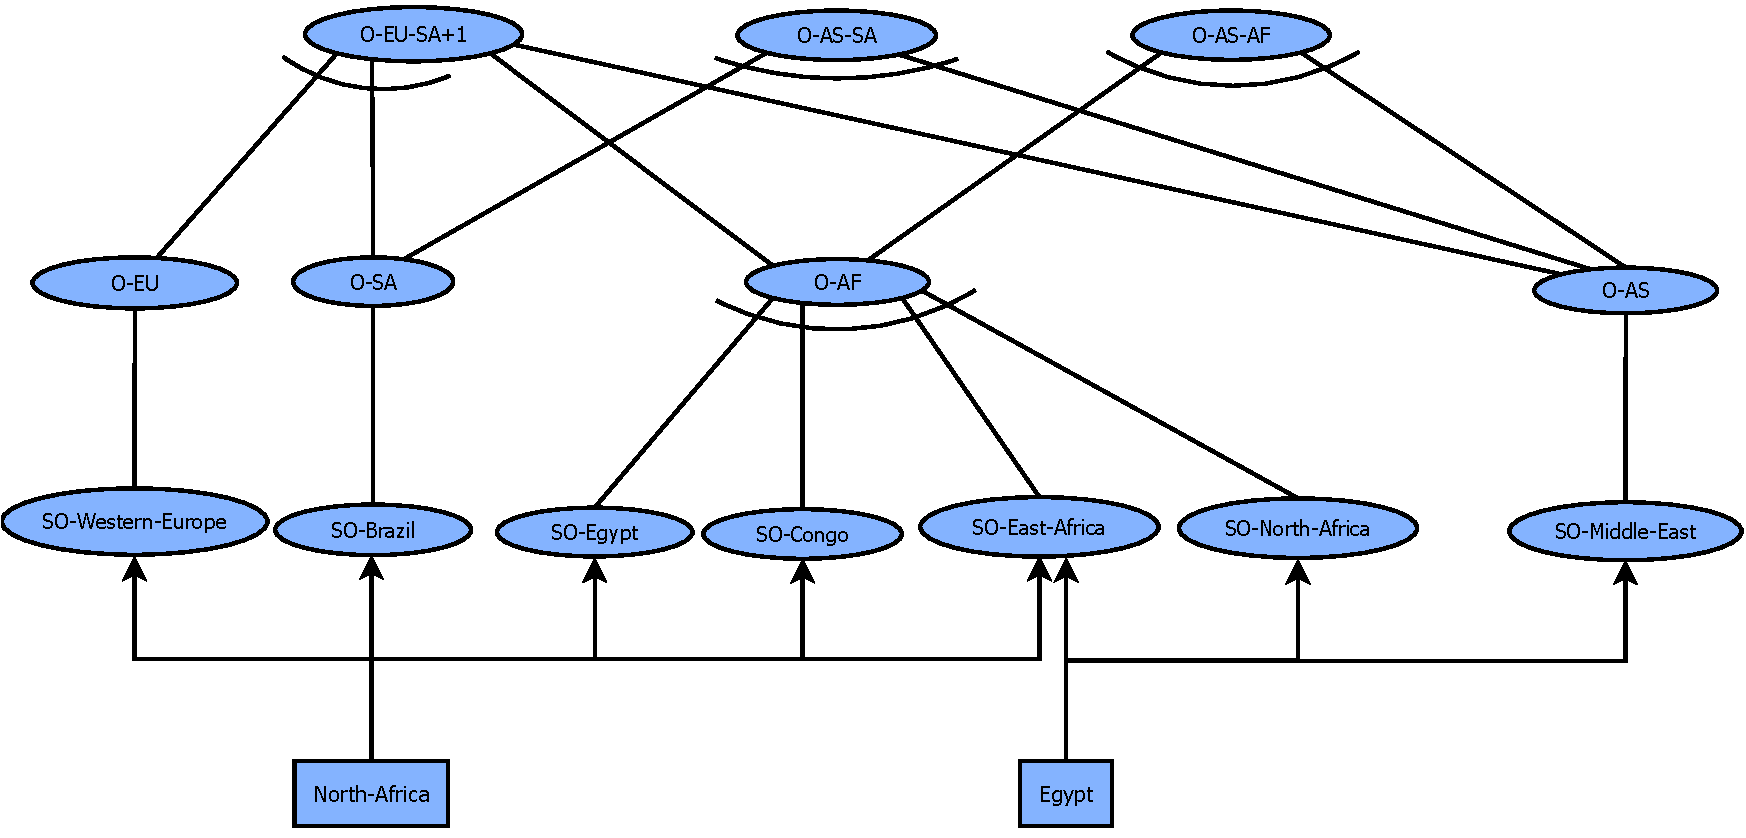
\includegraphics[width=\textwidth]{images/risk-plan-library.pdf}
}
\caption{Successful-Occupation Plan Library for North-Africa \& Egypt, \textbf{O} = Occupy, \textbf{SO} = Successful-Occupation}
\end{figure}

\newpage

The three root-goals of this environment are:

\begin{itemize}
\item
Occupy-Europe-South-America + One other continent (Occupy-EU-SA+1)
\item
Occupy-North-America-South-America (O-AS-SA)
\item
Occupy-South-America-Africa (O-SA-AF)
\end{itemize}

The first can be expressed in two ways given our example, therefore we must consider four root-goals. Each root-goal has a number of sub-goals. In the context of mission Risk, for a player to accomplish their root-goal they must have occupied every continent-sub-goal, this is done by performing Successful-Occupation actions on every territory contained in that continent. 

For the purposes of this example we introduce another notation which are squares that represent territory entities. Arrows away from these squares are connected to the actions a player can perform when occupying this territory. This is done to visualize the state of the world at the time the action was performed. For example by occupying the territory Egypt, allows a player to perform the actions: SO-East-Africa, SO-North-Africa and SO-Middle-East.

Recall the formulae:\newline

\centerline{
\textit{Pr(exp} $\wedge$ \textit{obs)} = \textit{Pr}(\textit{goals})\textit{Pr}(\textit{plans}|\textit{goals})\textit{Pr}(\textit{obs}|\textit{exp})
}

The term \textit{Pr}(\textit{goals}), the prior probability of each root-goal, is 1/\textit{n} where \textit{n} is the number of mission cards and therefore for this example is 1/3 for each root-goal. 

The term \textit{Pr}(\textit{plans}|\textit{goals}) is 1.0 as we always consider the the full set of root-goals hence removing the need to calculate a choice on the part of the player.

The term \textit{Pr}(\textit{obs}|\textit{exp}) is computed only when an observation occurs.

Player $p_1$ initially occupies the territory North-Africa and thus can perform actions connected to the North-Africa square. $p_1$ then performs a Successful-Occupation-Western-Europe action.

With an observation we can now compute the term \textit{Pr(exp} $\wedge$ \textit{obs)}, the probability of the explanation that the player has a root-goal and O-Western-Europe for $p_1$.

First we must compute \textit{Pr}(\textit{obs}|\textit{exp}), the probability that $p_1$ would choose to perform the observation O-Western-Europe given each root-goal.

\begin{itemize}
\item
Case 1 : \textit{Pr}(\textit{O-Western-Europe}|\textit{O-AS-AF})
\item
Case 2 : \textit{Pr}(\textit{O-Western-Europe}|\textit{O-EU-SA-AF})
\item
Case 3 : \textit{Pr}(\textit{O-Western-Europe}|\textit{O-EU-SA-AS})
\item
Cast 4 : \textit{Pr}(\textit{O-Western-Europe}|\textit{O-AS-SA})
\end{itemize}

The PR agent first applies the $computeExpProb$ operation for each of the above cases. Then using the $generatePS$ operation to builds a full pending set for $p_1$.

After this the PR agent retrieves a list of all consistent actions for each explanation by retrieving the $ECA$ set from each explanations data structure.

Given the observation O-Western-Europe, the complete pending set of the player, and the set $ECA$. The PR agent then uses the $computeObsProb$ operation to compute the probability of choosing the Successful-Occupation-Western-Europe action in the context of each root-goal.

For each root-goal the $computeObsProb$ filters out all action types except Successful-Occupation actions, from both $p_1$ pending set and the $ECA$ set. The result is the Successful-Occupation actions that are consistent with the explanation $expConAct$ and a new pending set $pTotalActNum$ which contain the following Successful-Occupation actions given the state of the world in this example:\newline

\centerline{
$p_1PS$ = \{SO-Western-Europe, SO-Brazil, SO-Egypt, SO-Congo, SO-East-Africa\}
}

Given these two sets we count the number of consistent actions that the players pending set contains for each respective root-goal, by comparing what actions are contained in $pTotalActNum$ to each root-goals $expConAct$ set. We also count the total number of actions a player can perform $pTotalActNum$.

In this example it is currently $pTotalActNum$ = 5

The counts given the action Successful-Occupation-Western-Europe is as follows:

\begin{table}[ht]
\centering
\begin{tabular}{|c|c|}
\hline 
\textbf{Explanation} & \textbf{Number of Consistent Actions} \\ 
\hline 
O-AS-AF & 3 \\ 
\hline 
O-EU-SA-AF & 5 \\ 
\hline 
O-EU-SA-AS & 2 \\ 
\hline 
O-AS-SA & 1 \\ 
\hline 
\end{tabular}
\caption{Consistent Action Count}
\label{table:consistent-action-count}
\end{table}

With these counts and our assumed $w$ the PR agent then computes a $base$ action probability for each explanation with the $computeBaseWeight$ operation as follows:

\begin{table}[ht]
\centering
\begin{tabular}{|c|c|c|c|}
\hline 
\textbf{Explanation} & Total-Weight & Left-Over & Base \ \\ 
\hline 
O-AS-AF & 0.02 * 3 & 1.0 - 0.06 = 0.94 & 0.188 \\ 
\hline 
O-EU-SA-AF & 0.02 * 5 & 1.0 - 0.10 = 0.9 & 0.18 \\ 
\hline 
O-EU-SA-AS & 0.02 * 2 & 1.0 - 0.04 = 0.96 & 0.192 \\ 
\hline 
O-AS-SA & 0.02 * 1 & 1.0 - 0.02 = 0.98 & 0.196 \\ 
\hline 
\end{tabular}
\caption{Consistent Action Count}
\label{table:territory-actions-bonus}
\end{table}

Consistent actions $cons$ are weighted so the probability of a consistent action $Pr(cons)$ = $base$ + $w$

Inconsistent actions $incons$ are not weighted so the probability of a inconsistent action $Pr(incons)$ = $base$

\begin{table}[ht]
\centering
\begin{tabular}{|c|c|c|}
\hline 
\textbf{Explanation} & $Pr(cons)$ & $Pr(incons)$ \ \\ 
\hline 
O-AS-AF & 0.208 & 0.188 \\ 
\hline 
O-EU-SA-AF & 0.2 & 0.18 \\ 
\hline 
O-EU-SA-AS & 0.212 & 0.192 \\ 
\hline 
O-AS-SA & 0.216 & 0.196 \\ 
\hline 
\end{tabular}
\caption{Computing Probabilities of Consistent/Inconsistent Actions}
\label{table:territory-actions-bonus}
\end{table}

The PR agent then computes an explanation that the players plan is the root goal given the observation \textit{Pr(exp} $\wedge$ \textit{obs)} by multiplying the term  \textit{Pr}(\textit{goals}) with one of the two action probabilities, depending on whether the action that was observed was consistent or not, in other words if was contained in $ECA$ or not.

For example to compute \textit{Pr(exp} $\wedge$ \textit{obs)} for the explanation O-EU-SA-AF the PR agent would choose to multiply by $Pr(cons)$ and so the calculation would be 1/3 * 0.2 

\begin{table}[ht]
\centering
\begin{tabular}{|c|c|c|}
\hline 
\textbf{Explanation} & \textbf{Terms Multiplied} &\textit{Pr(exp} $\wedge$ \textit{obs)} \\ 
\hline 
O-AS-AF & \textit{Pr}(\textit{goals}) * $Pr(incons)$ & 0.0626 \\ 
\hline 
O-EU-SA-AF & \textit{Pr}(\textit{goals}) * $Pr(cons)$ & 0.0666 \\ 
\hline 
O-EU-SA-AS & \textit{Pr}(\textit{goals}) * $Pr(cons)$ & 0.706 \\ 
\hline 
O-AS-SA & \textit{Pr}(\textit{goals}) * $Pr(incons)$ & 0.0653 \\ 
\hline 
\end{tabular}
\caption{Computing Un-Normalised Root-Goal Probabilities}
\label{table:territory-actions-bonus}
\end{table}

\newpage

Finally to complete the calculation of \textit{Pr(exp}|\textit{obs)} the PR agent normalises each with the following formula: \newline

\centerline{
\textit{Pr($exp_0$}|\textit{obs)} = \textit{Pr($exp_0$} $\wedge$ \textit{obs)} / $\displaystyle\sum\nolimits_{i}$ \textit{Pr($exp_i$} $\wedge$ \textit{obs)}
}

For example to compute \textit{Pr($exp$}|\textit{obs)} for O-EU-SA-AF, the PR agent would first sum all explanation probabilities which is:

0.0626 + 0.0666 + 0.0706 + 0.0653 = 0.2651 

It would then divide the probability of the term \textit{Pr($exp$}|\textit{obs)} for the O-EU-SA-AF root-goal which is:

0.0666 / 0.2651 = 0.251.

\begin{table}[ht]
\centering
\begin{tabular}{|c|c|c|}
\hline 
\textbf{Explanation} &  \textit{Pr($exp$}|\textit{obs)} Pre-Normalisation &  \textit{Pr($exp$}|\textit{obs)} Post-Normalisation \\ 
\hline 
O-AS-AF & 0.0626 & 0.236  \\ 
\hline 
O-EU-SA-AF &  0.0666 & 0.251 \\
\hline 
O-EU-SA-AS &  0.0706 & 0.266 \\ 
\hline 
O-AS-SA & 0.0653 & 0.246 \\ 
\hline 
\end{tabular}
\caption{Consistent Action Count}
\label{table:territory-actions-bonus}
\end{table}

At this point we set each normalised value of \textit{Pr($exp$}|\textit{obs)} as the value of each explanation and choose the highest as the prediction of the PR agent. This is done to keep the explanation values from dropping to zero too quickly.

Failed-Occupation actions are computed in the exact same way as Successful-Occupation actions, the difference being that the pre-defined $w$ is set to a lower value than that of Successful-Occupation.

The computation of other actions in the environment is considerably simpler given the assumptions of the model. To compute defence and movement actions the PR agent would first retrieve the current explanation probability. Then firstly taking into consideration, whether it was an action performed on a territory that was contained in the high-level root-goal. If so then whether the action was consistent or not it would multiply it by for example:

\begin{itemize}
\item
1.02 for consistent actions.
\item
0.98 for in-consistent actions.
\end{itemize}

The final computed probability would then again be normalised and set to the current explanation probability as normal.

For reinforce actions the PR agent considers each explanations, if the reinforce action is observed as consistent the current explanations probability is multiplied by 1.02 if inconsistent then it is multiplied by 0.98. 

\section{Summary}

Environmental modelling and a design of environment data structures was necessary in order to allow the PHATT algorithm to operate in the Risk environment. 

Each action in the Risk environment was modelled and various assumptions about each were made in-order to compute the probability of a player. Where necessary data structures were designed for the most significant objects in the environment. The purpose of each data structure would be to contain the essential information required by the PR agent.

A key concept in the design of the agent, is that the pending set of a player is decided \textit{a priori} by the territories that a player owns. And by combining the actions that are possible from each territory that a player owns into a single set, all the actions a player can perform can be captured.

\chapter{Implementation}

The Java programming language was selected for the implementation of the PR agent. The reasons for doing so were:

\begin{itemize}
\item
The availability of an open-source project with an active development team.
\item
Personal familiarly with the language.
\item
Java being cross-platform.
\end{itemize}

\section{System Architecture}

\begin{figure}[h]
\centerline{
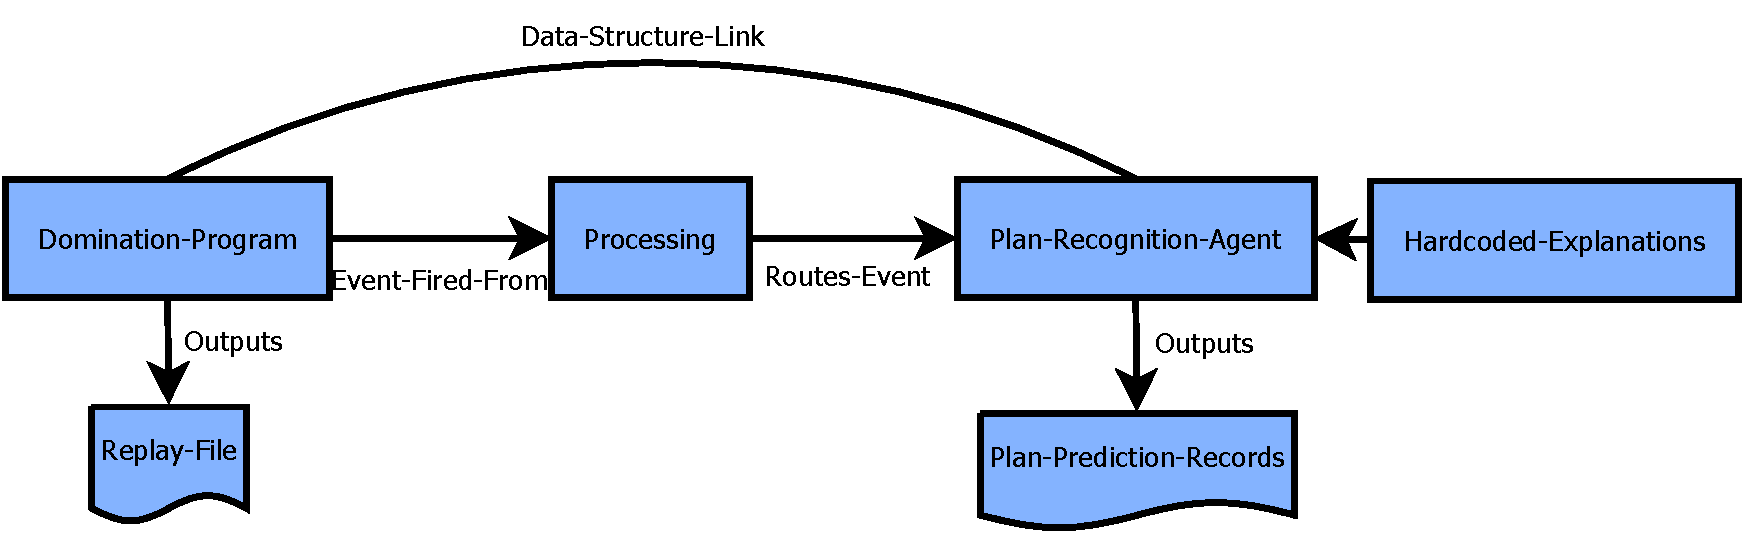
\includegraphics[width=1.2\textwidth]{images/system-architecture}
}
\caption{System Architecture}
\end{figure} 

The system followed an \textit{event-driven} architecture, comprising of three major components.

The \textit{Domination-Program} which refers to the open-source game developed by Yura.Net. Modifications to the source code of the program were:

\begin{itemize}
\item
Automating the output of the \textit{Replay-File}.
\item
Code to fire events into the \textit{Processing} component. 
\end{itemize}

The \textit{Processing} component was responsible for routing events to the \textit{Plan-Recognition-Agent}.

The \textit{Plan-Recognition-Agent} as well as being responsible for had access to the data structures in the Domination program. Rather than storing its own copy avoided any synchronisation between it and the Domination program. Additionally the advantages of this approach includes less overhead as well significantly reducing the possibility that the PR agents copy loses synchronisation with the Domination-Programs data structures. On the other hand a disadvantage is that this makes the plan-recognition-agent more dependant on the methods of the developers implementation.

The PR agent made extensive use of the freely available Google Guava libraries. These allowed the prediction agent to operate concurrently with the game as well as more efficiently in its operations.

A set of explanation objects made up the \textit{Hard-coded-Explanations}. Explanation objects had hard coded root and sub goals. Using these sub-goals, the system could build a list of consistent and inconsistent actions using the data structures stored by the Domination program. 

The \textit{Hard-coded-Explanations} were implemented as separate to the core structure of the PR agent. As given a complete list of hard-coded explanations for another map the plan recognition can be used successfully once again.

The Domination-Program is capable of outputting a Replay-File that could be used to replay a game.

The PR agent would output a csv file containing the plan predictions for each player over the course of the game.

The architecture of the system is such that the PR agent is not as dependant sub-component of the game, but rather a separate entity that operates in parallel to the game which if need be could be replaced by another implementation of a PR agent.

\newpage

\section{Plan Recognition Agent Architecture}

\begin{figure}[h]
\centerline{
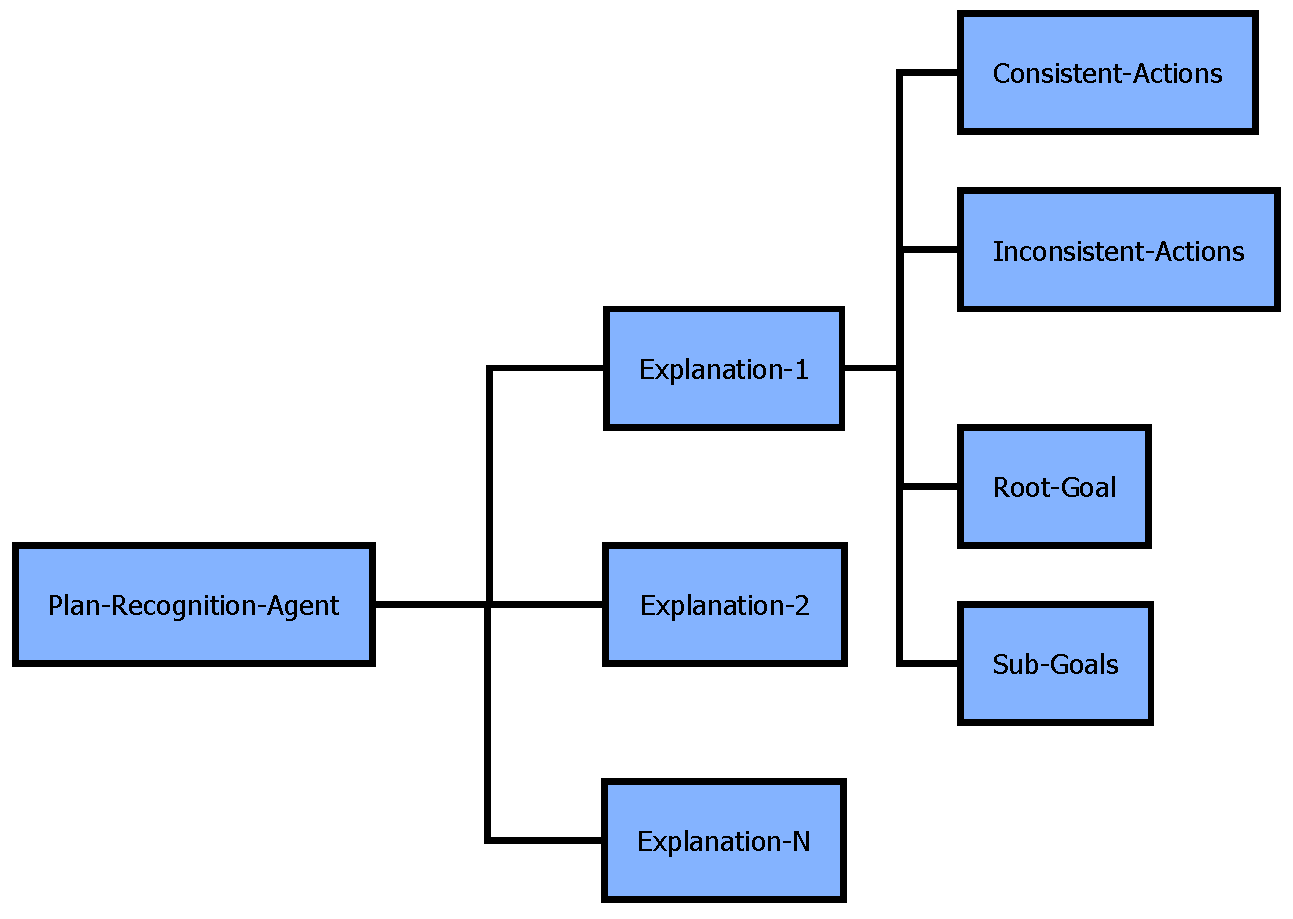
\includegraphics[width=0.7\textwidth]{images/plan-recognition-agent-architecture}
}
\caption{PR Agent Architecture}
\end{figure} 

The Plan-Recognition-Agent has a data structure for each player, which in turn has several explanation data structures that are initially hard-coded. Each explanation object calculates its own probability.

The Root-Goal and Sub-Goal data structures must be hard-coded 

When an event arrives from the processing class it is routed to its specified player data structure and then to its specified explanation data structure which would use the observed action to compute its new probability.

Data structure that stores the probabilities of each players explanation structure once this game ends the data structure writes it out to a data folder as a csv file.

\newpage

\section{Event Design}

To operate the PR agent needs to be aware of several aspects of the game. In particular: how many players there are, when the game begins, the games initial state, any changes that occur in the game and when the game is finished. These aspects can be broken down into individual events:

\begin{itemize}
\item
Start Game
\item
Player Initialisation
\item
Player Removal
\item
Territory Placement
\item
Successful Occupation
\item
Failed Occupation
\item
Army Movement
\item
Reinforcement
\item
End Game
\end{itemize}

When these events occur a distinct event object is fired, these even objects contains important information about the event that is necessary to the PR agent. These events are observed by the processing class which then routes them to the PR agent. The PR agent then looks at the received event object(s) and depending on the type of event object and the information held by it, handles the object appropriately. The types of events, what they contain and their purpose are:

\begin{table}[ht]
\centerline{
\begin{tabular}{|c|p{6cm}|p{8cm}|}
\hline 
\textbf{Event Type} & \textbf{Contains Variables} & \textbf{Purpose} \\ 
\hline 
New-Player & player-name & Initialises a new player data structure with ID \textit{player-name}. \\ 
\hline 
Remove-Player & player-name & Destroys the player data structure with ID \textit{player-name}. \\ 
\hline 
Successful-Occupation & attacker-name, cName, tName & Signals that the player named \textit{attacker-name}  performed a Successful-Occupation. \\ 
\hline
Failed-Occupation & attacker-name, cName, tName & Signals that \textit{attacker-name} performed a Failed-Occupation. \\ 
\hline
Successful-Defence & defender-name, cName, tName & Signals that \textit{defender-name} performed a Successful-Defence. \\ 
\hline
Failed-Defence & defender-nName, cName, tName & Signals that \textit{defender-name} performed a Failed-Defence. \\ 
\hline
Army-Movement & player-name, cName, tName & Signals that \textit{player-name} performed an Army-Movement. \\ 
\hline
Reinforce & player-name, cName, tName & Signals that \textit{player-name} performed a Reinforce action. \\ 
\hline
\end{tabular}
}
\caption{Event Object Specification, c = Continent, t = Territory}
\label{table:event-description}
\end{table}

More specifically other than player initialisation or removal events, each event will trigger the computation of explanation probabilities, which players explanation probabilities are decided for example by the \textit{attacker-name} and what effect, is decided by the state of the Risk world namely the respective players pending set which can be built from the data structures of the Domination-Program and the continent and territory name of the event.

\section{System Operation}

Before a game begins, based on the players registered in the game lobby screen the PR agent initialises a set of player data structures. 

The PR agent first initialises the list of \textit{Hardcoded-Explanations} which involves building the set of consistent and inconsistent actions based on the explanations sub-goals. These explanation objects contain all the necessary information from the environment to computes its own probability. Once the complete list of explanations has been fully initialised it is cloned into each players data structure.

Once action events start firing from the Domination-Program and was routed by the Processing component, the Plan-Recognition-Agent will depending on the event compute new explanation probabilities for a player.

This would continue till the end of a game the domination program as well as the PR agent would output two files allowing the replay of a game and a record of the PR agents prediction probabilities for each players explanations over the course of the game.

\section{Summary}

The Plan-Recognition-Agent was written in the Java programming language following an event-driven system architecture. It was built to be able to operate on any map developed for the Domination-Program and using the Google Guava libraries could operate in parallel to the Domination program. 

By receiving events fired from the program it would update locally held player data structures that contained information about each players explanation predictions and any other required would be retrieved from the Domination-Program.

At the end of a game the Plan-Recognition-Agent would output two files. One was a Replay-File that would allow a complete replay of the game, the other was the Plan-Prediction-Record which detailed the probabilities of each players explanations over the course of the game.

\chapter{Evaluation}

The evaluation plan consists of four experiments on the Plan Recognition agent:

\begin{enumerate}
\item
Free Play
\item
Constrained Play
\item
A.I Play - 100
\item
A.I Play - 4
\end{enumerate}

\section{Experimental Format}

\subsection{Participant Experiments}

Of the four experiments, two were conducted with human players: 

\textit{Free Play}, where human players "play to win", in any manner they see fit. This is how people would normally play mission Risk.

\textit{Constrained Play} consists of players only performing actions that are \textit{directly-consistent} with their root-goal. 

An example of a directly-consistent action is occupying a territory required by a root-goal. An example of the converse, a \textit{indirectly-consistent} action, would be breaking another player's continent by occupying a territory in that continent. It is indirectly-consistent because whilst not satisfying the player's goal, it prevents other player's from satisfying theirs. And only one player can win. 
More formally, given a set of actions (excluding card related actions), a player will only either:

\begin{itemize}
\item
Choose to attack a territory that is directly-consistent with their plan, or a territory that is on the shortest route to a territory that is directly consistent with their plan.
\item
Reinforce a territory that is directly-consistent with their plan, or a territory that is on the shortest route to a territory that is directly consistent with their plan.
\item
Moves armies to a territory that is directly-consistent with their plan, or a territory that is on the shortest route to a territory that is directly consistent with their plan.
\end{itemize}

This artificial form of play is designed to give optimal performance from the plan recognition agent. This is achieved by minimizing environmental noise from indirectly-consistent and inconsistent actions found in the other forms of play. Under this form of play, a high prediction accuracy is expected. If this is not the case then the resulting experiments should provide a good indication as to why.

The A.I. players used were those provided with the Domination implementation of Risk. For experiments involving human players, the game rules were explained before the start of the experiment. 

For constrained play, the particular play style required was described to participants.

For free play, it was made clear to participants that there were two primary methods of winning the game:
\begin{enumerate}
\item
Eliminating all other players from the game.
\item
Completing their mission card.
\end{enumerate}

At the end of the game participants were asked to give a short summary of their initial plan and any changes they to it during the course of the game. 

In total, nineteen people participated in the experiments. Some took part multiple times.

The final count of participant data samples was:

\begin{itemize}
\item
75 data samples collected for free play.
\item
100 samples collected for constrained play.
\end{itemize}

\subsection{A.I. Experiments}

\textit{A.I. Play} are games played using only the game A.I provided with the Domination Risk implementation. These A.I. players can be substituted for human players to the point where a game can consists of only A.I. players battling each other. A.I. games can finish in a fraction of the time that it takes to complete a game with human players.

According to the A.I developer at Yura.Net, "the mission A.I. is a minimal extension of the core play. Since the core logic is reasonably good at conquering continents and eliminating opponents it just has it's decisions skewed a little to make sure it's going after the right continent/player without causing it to generally play poorly."

Looking at the Domination program, the degree to which the A.I.'s decisions are skewed, is dependant on a variable $w$. By increasing this value, it causes the A.I. to more actively pursue its assigned mission card.

Using this we can evaluate the plan prediction accuracy of the PR agent, and perhaps more importantly see whether the PR agent is capable of detecting the behavioural change that follows a change in $w$.

Automating the collection of these data samples using the free macro program AutoHotkey, provided an opportunity for the collection of a large number of data samples for analysis.

The final count of A.I. data samples was:

\begin{itemize}
\item
1004 A.I. data samples set at $w$ 4.
\item
1004 A.I. data samples set at $w$ 100.
\end{itemize}

\newpage

\section{Data Collection}

After a game had finished the Domination program would generate a replay file. This file can be loaded later through a specialised interface, allowing an exact replay of the game.

\begin{figure}[h]
\centerline{
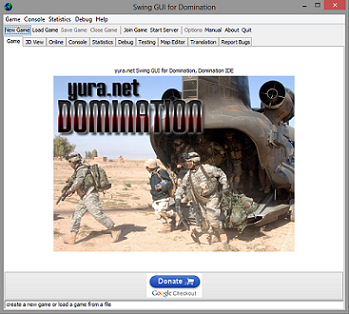
\includegraphics{images/domination-debug-gui.png}
}
\caption{Domination Debug Graphical User Interface}
\label{fig:dom-debug-gui}
\end{figure}

Using this tool made it possible to re-observe games for their evaluation. It also allows the PR agent to be tested with different modelling and calibrations in the same game twice. This eliminates environmental variables between comparisons of the PR agent.

In addition to the Domination replay file, the PR agent would also generate a CSV file containing the significant features of a game, namely:

\begin{itemize}
\item
Which players took part
\item
Which player won
\item
Each player's mission card
\item
The probabilities of each player's explanations over the course of the game
\end{itemize}

Scripts written in Python were used to automate the analysis of the generated CSV files.

\newpage

\section{Experimental Findings}

Experiments with the PR agent revealed the following insights:

\begin{enumerate}
\item
The prediction accuracy of the PR agent is highest in constrained play.
\item
The prediction accuracy of the PR agent is higher for winning players than losing players. 
\item
The prediction accuracy of the PR agent is higher for human players than the Domination A.I. players.
\item
The prediction accuracy of the PR agent reflects the failings of the Domination A.I. in completing its mission.
\item
There is a positive correlation between game length and prediction accuracy. 
\item
This is most true of winning players. 
\item
Constrained play games were never longer than 120 turns, making them the shortest of the four game types.
\end{enumerate}

Keeping in mind the initial hypotheses, we attempt to evaluate the claim that plan recognition algorithms are beneficial in Risk.

To do this, we explore the two questions that define what we consider beneficial:
\begin{itemize}
\item
Is the PR agent accurate in its predictions?
\item
How quickly does the PR agent converge on a correct prediction?
\end{itemize}

The term \textit{General} player is used to refer to both human and A.I players. Players are further decomposed into players who won, \textit{Winners}, and players who lost, \textit{Losers}.

\subsection{Format of Explanation Convergence}

At the start of a game, forty two turns are required to place one army on each territory of the Risk map. These observations are not taken into account by the PR agent, as the distribution of territories between players is automatic and random.

After this, the remaining initial armies are distributed by players onto their territories. During this, the probability of explanations that are consistent with a player's actions will slowly increase. Conversely, those explanations with which the actions are inconsistent with will slowly decrease.

Once the initial setup is complete (which ranges from 80 to 120 turns, depending on the number of players), the attack phase begins for the first player $p_c$. At this time the probabilities of $p_c$ explanations may change rapidly, depending on the number of actions that $p_c$ performs in their turn.

The most significant change in explanation probability occurs when there are many Successful-Attack actions in a single turn. This is due to the design of the PR agent.
After $p_c$'s turn is over, other players begin their attack phases in turn. Unless the action another player performs is to attack a territory owned by $p_c$, the probabilities of $p_c$ explanations remained unaffected.

This pattern continues till the end of the game, at which point the PR agent will have determined its predictions. The level of convergence differs between types of play, although generally significant convergence only occurs after the attack phases have begun.

\newpage

\subsection{Prediction Accuracy in General}

\begin{figure}[h]
\centerline{
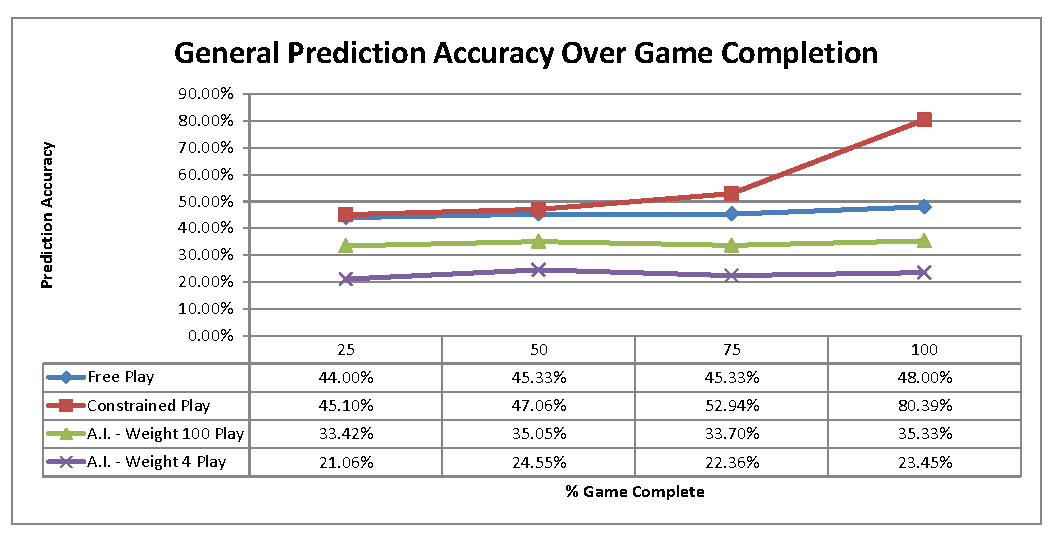
\includegraphics[width=0.9\textwidth]{images/general-game-complete.pdf}
}
\caption{General Prediction Accuracy}
\label{fig:dom-debug-gui}
\end{figure}

\begin{figure}[h]
\centerline{
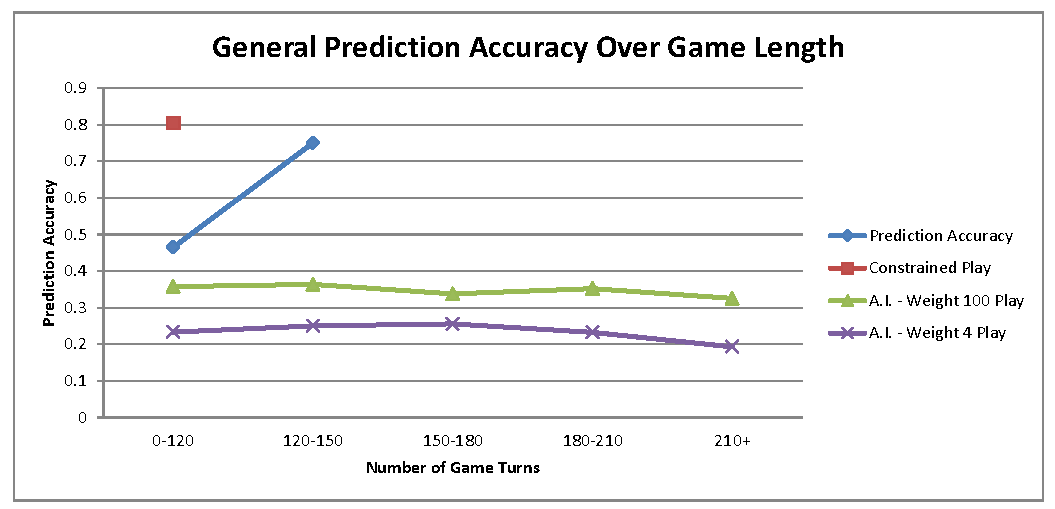
\includegraphics[width=0.9\textwidth]{images/general-game-length.pdf}
}
\caption{The general prediction accuracy of the PR agent at various game lengths. }
\label{fig:dom-debug-gui}
\end{figure}

The data has several trends with regards to player prediction accuracy. 

The PR agent plan prediction accuracy was significantly better in \textit{Constrained play than in Free or A.I. play} in both interval of game completion, and game length metrics. This is unsurprising given its artificial nature. Designed to be ideal the scenario for the PR agent, it is not a good measure of evaluating the success of the PR agent in general. Instead, in conjunction with Free Play, it gives us a better picture of how well the PR agent performs on human players.

The PR agent's plan prediction accuracy was on average better for human players than A.I. players. The reason for this is the degree with which human and A.I. players actively follow their mission card. The data suggests that, since the core A.I. is a modification to the domination mode A.I., it is not specifically built to actively follow a plan. Thus we can confirm that human players followed their mission cards more actively than A.I. players.

Comparing the prediction accuracy at $w$4 and $w$100, we see up to a 10\% improvement in the plan prediction accuracy of the PR agent. This confirms that as the A.I.'s decisions become more skewed towards occupying mission continents and less towards other activities, prediction accuracy increases. 

There is a 25\% increase in the plan prediction accuracy of the PR agent for constrained play in the 75\% to 100\% game completion category. In general there is a rise in the prediction accuracy in this game completion category across all forms of play, though the most significant rise remains exclusive to constrained play. Again, this is likely due to the nature of constrained play. As we shall see with further analysis of winners and losers, both categories of constrained play yield high prediction accuracy.

A trend can be seen of an increase in plan prediction accuracy towards the end of a game. As before, this is primarily due to how winners perform a large number of consistent actions in a short span of time at the end of a game.

We can look at an example of constrained play to confirm this.

\begin{figure}[h]
\centerline{
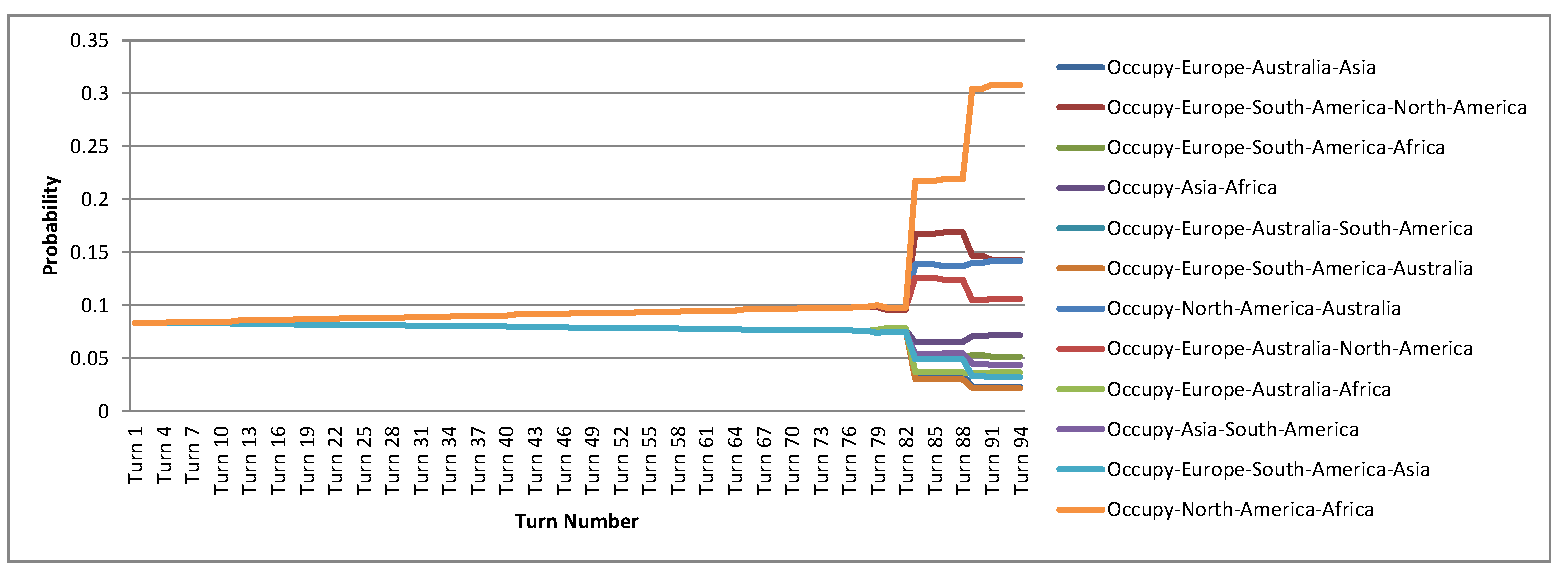
\includegraphics[width=1.1\textwidth]{images/short-constrained-game.pdf}
}
\caption{A.I. 4 - Example Game}
\label{fig:dom-debug-gui}
\end{figure}

The winning players mission was to capture North-America and Africa. For the majority of the game - during the placement phase and up until turn 82 - the probability does not rise significantly. After turn 82, when the attack phases begin, the increase in explanation probability is substantial. Convergence to the correct explanation occurs within 10 turns, reaching a significantly higher explanation probability soon after attacks have begun.

The general prediction accuracy over game length falls for A.I. players over time, whereas for human players it increases. Figure 5.2 does not echo this trend though which indicates that prediction accuracy over game length appear to be stable which is indicative that the number of samples from Figure 5.3 reaching game length of over 210+ are relatively small as to not affect the average accuracy so significantly.

The of length the human games ranged between 120 and 150 turns, which is far lower than that of A.I. games. This suggests that either:
\begin{itemize}
\item
The A.I. is good at preventing other A.I. players from winning. 
\item
Games are longer because the A.I. is ineffective at finishing their mission.  
\end{itemize}

With an example we can see evidence to suggest the latter point. 

\newpage

\begin{figure}[h]
\centerline{
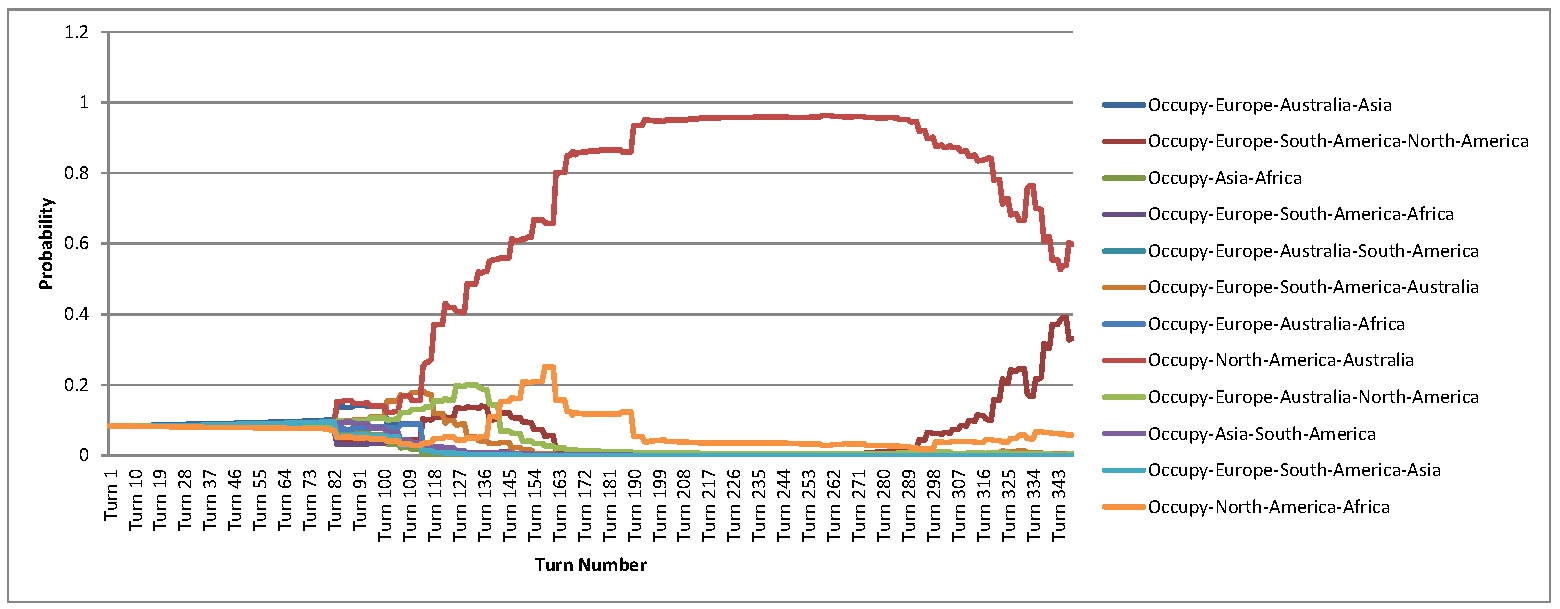
\includegraphics[width=1.1\textwidth]{images/bad-long-game.pdf}
}
\caption{A.I. 4 - Example Game}
\label{fig:dom-debug-gui}
\end{figure}

Figure 5.5 illustrates the probabilities of explanations for a 4 player game between A.I.s. Player 4,  who has the mission of conquering Asia and South-America, won in approximately 342 turns. The A.I. players were caught in a stalemate between each other for many turns, arguably not out of skill but by a lack of strategic diversity. 

For instance, they make no attempt to fortify and hold continents when they were weak, or to consolidate their armies in strategic territories. Instead, the players opted for a strategy of all-out attack. Most of player 4's engagements occurred in North-America and Australia - continents outside of its mission. At one point, the player had a clear advantage but chose to attack a non-mission continent to eliminate a weaker player instead of taking Asia, its final mission continent. 

This observation coincides with the significant drop of the PR agents prediction accuracy for A.I. - 4 games longer than 210 turns. The number of such examples must be relatively small because we do not see a significant drop in prediction accuracy of A.I -4 games between 75 to 100 \% game completion.

\newpage

\section{Plan Recognition Agent Winner Prediction Accuracy}

\begin{figure}[h]
\centerline{
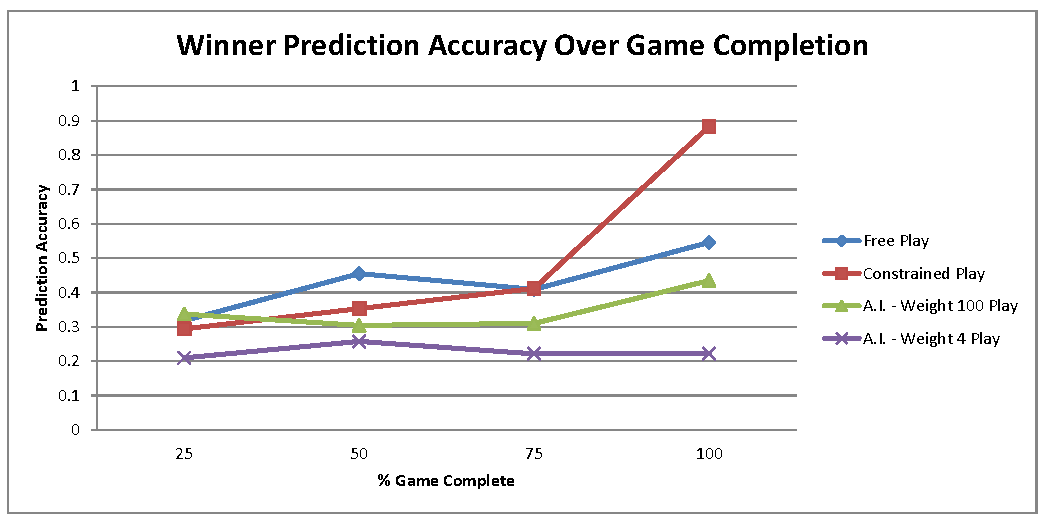
\includegraphics[width=0.9\textwidth]{images/winner-game-complete.pdf}
}
\caption{Winner Plan Prediction Accuracy}
\label{fig:winner-pred-accuracy}
\end{figure}
\begin{figure}[h]
\centerline{
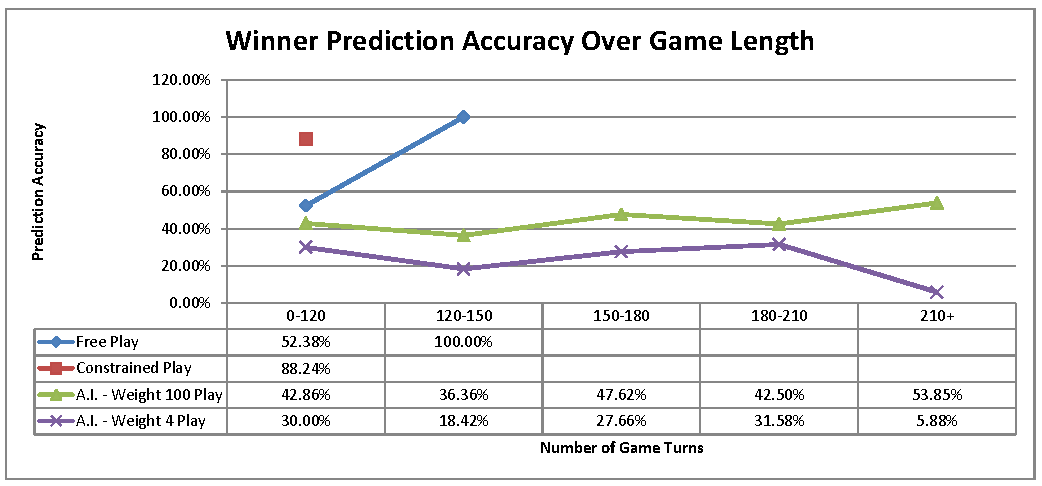
\includegraphics[width=0.9\textwidth]{images/winner-game-length.pdf}
}
\caption{Winner Plan Prediction Accuracy}
\label{fig:win-plan-pred}
\end{figure}

First, we must point out that the prediction accuracy of the PR agent is 1.0 only due to the number of data samples of winners being small. There was only a single data sample of a winner between 120-150 turn long game, and that sample was correctly predicted.

Games of constrained play were never longer than 120 turns.

The highest plan prediction accuracy of the plan recognition is 88.24\%, which is for winners in constrained play games of length 0-120.

What is striking about the data for winners, is that for A.I. - 4 games, there is a significant drop in plan prediction accuracy from 31.58\% to 5.88\% in from the 180-210 to the 210+ game length category.

As we saw from the example of a long A.I. game in the previous section, this can be explained by the majority of the losers having been eliminated at that stage and the winner was focused on eliminating the last player. This involved performing many inconsistent actions to eliminate them, and the losers that did survive did not perform many actions because of a comparatively low level of reinforcement armies. Once again, though the number of these cases are small given the winner’s plan prediction accuracy remains stable on average through a game.

For A.I-100,  there is a positive trend that as the game length increases, so does the plan prediction accuracy.

The trend of increase towards the end of the game is much more apparent for winners, as seen by significant increases of plan prediction accuracy between 75\% and 100\% game completion. This is due to winners performing more directly-consistent actions at the end of a game.

There are cases where winners have occupied an entire continent and completed their mission in one turn. Since sampling is done on a turn by turn basis, the PR agent will miss the significant change in probabilities. This is a consequence of the system not registering an end of turn, but rather a different event which is the end of the game.

\newpage

\section{Plan Recognition Agent Loser Prediction Accuracy}
\begin{figure}[h]
\centerline{
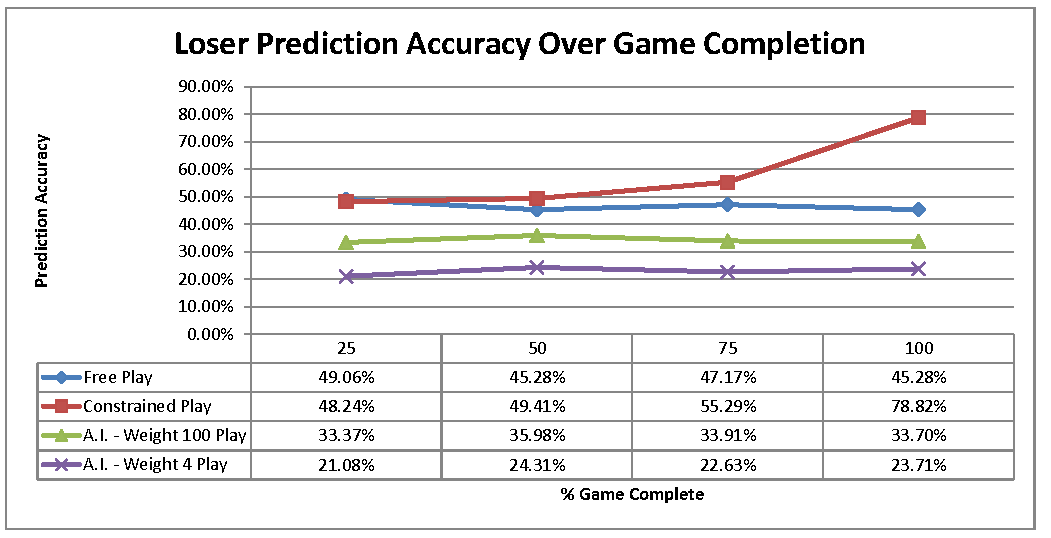
\includegraphics[width=0.9\textwidth]{images/loser-game-complete.pdf}
}
\caption{Loser Plan Prediction Accuracy}
\label{fig:dom-debug-gui}
\end{figure}

\begin{figure}[h]
\centerline{
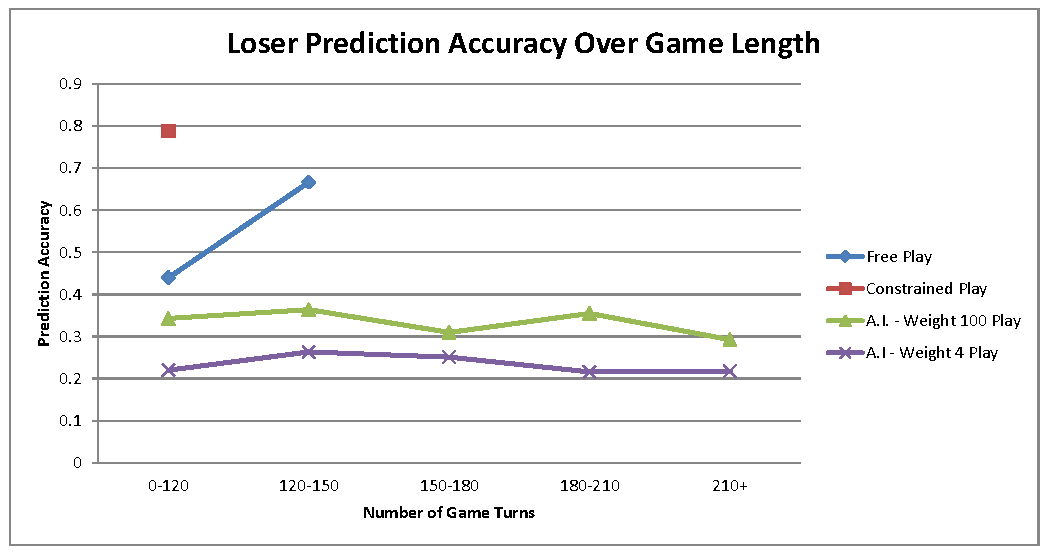
\includegraphics[width=0.9\textwidth]{images/loser-game-length.pdf}
}
\caption{Winner Prediction Accuracy}
\label{fig:dom-debug-gui}
\end{figure}

\newpage

Losers in A.I - 100 appear to show negative trend in that as the game length increases the prediction accuracy falls. As we saw from an analysis of winners the inverse to this was true, as game length increases the plan prediction accuracy increases as well. This is an interesting correlation as it suggests that the prediction accuracy of winners at least for A.I. - 100 play gets better as losers get worse. This makes sense; by definition, a loser cannot complete their mission. 

Losers are often prevented from successfully achieving their goal as they may be eliminated early or may be pushed out of their mission continents. The following is an example of a player with the mission of taking North-America and Africa being eliminated from a game at approximately turn 75.

\begin{figure}[h]
\centerline{
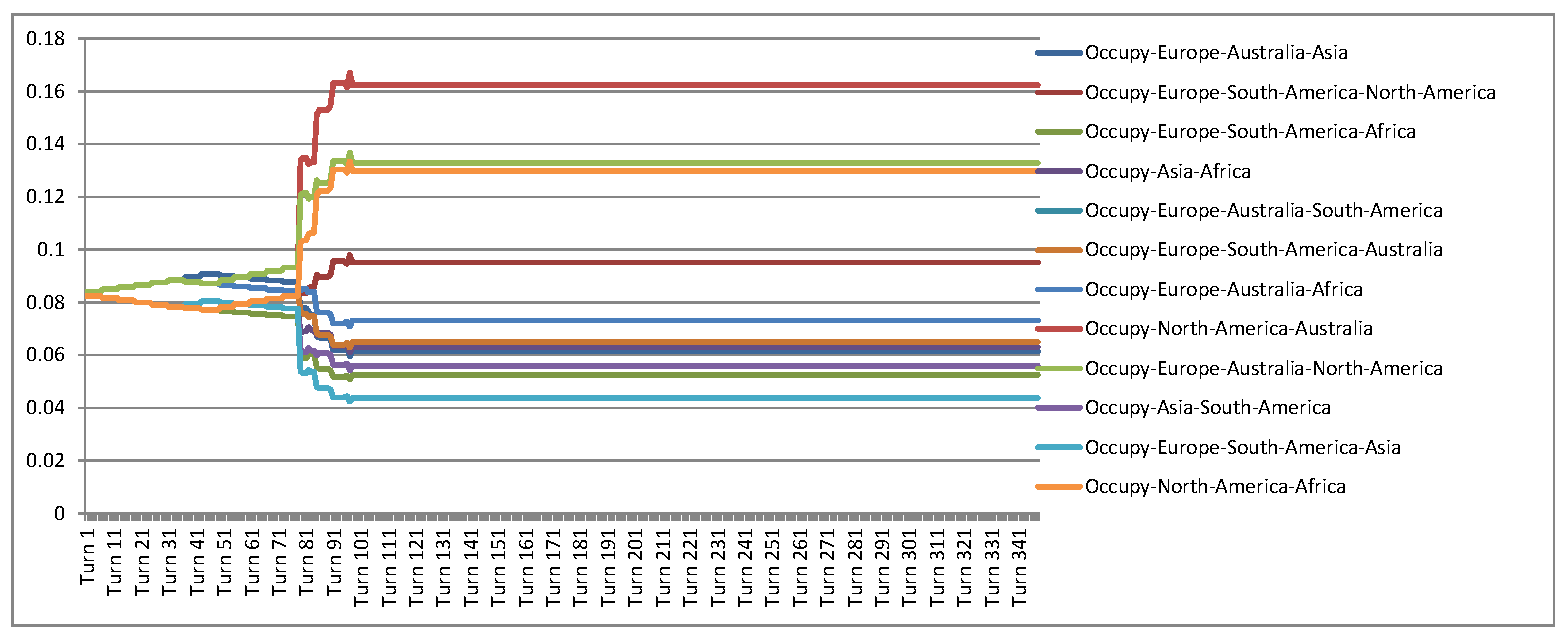
\includegraphics[width=1.1\textwidth]{images/player-elim-early.pdf}
}
\caption{Example Player Eliminated}
\label{fig:dom-debug-gui}
\end{figure}

\newpage

A number of incorrect predictions occurred due to the lack of data about players that are eliminated early on. If a loser is eliminated early in the game, then their explanations probabilities would \textit{flat-line}. This can be seen clearly in Figure 5.10. If the loser had been performing more inconsistent actions than consistent actions up to that point, then the prediction will be incorrect and will remain so for the rest of the game. Conversely, it may remain correct for the same reason.

\section{Outcomes}

The PR agent has shown to perform better than uniform choice of mission card, but the prediction accuracy is still below 50\% and significant successful convergence does not occur typically until after 75\% of the game is complete. This does not meet the projects definitions of beneficial. In defence to this, the PR agent did perform better on players than on A.I. which for our purposes is significant. 

The data that we have collect supports the theory that unless players behaved as in constrained play, the intense adversarial atmosphere, together with the high level of overlap between mission cards causes significant noise for the PR agent, which is detrimental to converging on the correct explanation but rather results in on average high levels of incorrect plan prediction's.

Particularly difficult areas of this project have been, deciding on methods of computing action probabilities and how much if any to weight each of those actions. 

There was trouble working with an algorithm that was made to deal with an action space rather than such a significant state based environment. Therefore having to figure out how to represent the environment as an action space so that the algorithm could operate was particularly difficult. 

Finding plan recognition algorithms that are made to cope with such noisy environments may be beneficial in future research. Also given that it works well in constrained play, the design has some in less complex environments such as the card game Pit.

Constrained play games were never longer than 120 turns, thus making them the shortest of all game types. In constrained play, players do not purposely seek to hinder the progress of other players' missions. So therefore winner of constrained play  tends to be the player with the least overlapping missions with other players, and the smallest number of territories to occupy. This situation allows for a player to quickly complete their mission with little opposition from other players who do not interfere due to the design of constrained play. Hence games are shorter.

For A.I. 100 there is a inverse correlation between the plan prediction accuracy of winners and the plan prediction accuracy of losers. 

Winners by definition have successfully performed their mission or will have eliminated every player, in either case they will have performed each consistent action for a mission at least once. Making on average as the data reflects the number of consistent actions performed by the winner, on average higher than that of losers hence making it easier to detect. This proposition is supported by how the PR agents \textit{prediction accuracy of winners is better than that of losers}.

In Risk.there is only one winner. Risk is an adversarial environment where right from the start you are attacked. Given that you can survive an onslaught of attacks in-order to achieve ones own mission, players must either directly or indirectly eliminate each other and often modify their own plan in order to continue surviving or prevent other players from winning. 

Given the design of the PR agent these changes in behaviour are see as directly-inconsistent with their own mission and rather seems consistent with whatever explanation that those actions \textit{are} directly-consistent with instead.

It is unfortunate that the project has not proved the original hypothesis though how indeed showed som success. And we can conclude, that Risk is certainly a challenging environment to perform plan recognition for.

\section{Future Work}

A platform has been setup for further improvements of the PR agent. Avenues of future work include exploring:

If the plan prediction accuracy of winners is better than loser is in fact may be due to because weighting of attack actions is towards successful attacks, of which winners perform more. This question can be explored.

The effects on accuracy when experimenting with A.I. play was done with six players. This would be interesting to see the effects on prediction accuracy differs depending on the numbers of players in the game.

Data has been collected for explanation accuracy measure but has not been analysed. Doing so could shed some light onto whether the accuracy of mission cards are different and why.

Using the collected data samples, test the PR agent with different models of the environment or different calibrations.

The model could be extended to include other mission cards.

\subsection{Improvement of Action Probability Computation}

Currently the system suffers from the problem of distinguishing noise from meaningful actions. Solving this problem could be tackled in two ways:

\begin{itemize}
\item
Identifying actions are indirectly-consistent and modelling them to accurately contribute to explanations - further modelling to further differentiate noise from meaningful behaviour.
\item
Making the meaningful actions that one can already identify greater significance to actions that are directly consistent through the state of the game more significant - making noise less significant.
\end{itemize}

Considering the latter point. By knowing that a player owns four out of five of a continents territories when they choose to attack the last territory is intuitively more significant to the explanation of the player wanting to own that continent then if they only owned a single continent of that territory and choose to attack another territory.

Currently the weight for actions is flat at the moment or more precisely actions are consistent in themselves but may not be consistent given the \textit{context} of the game state. To deal with this, we propose using a dynamic weight system that captures certain aspects of the Risk environment as follows:

Explanation-Prob = Explanation-Prob * Weight * Fraction-Representing-State-of-Environment

More specifically:\newline

\centerline{
Weight = 0.1 * 1- (No of Consistent actions) * (No of territories a player owns of that continent)
}

Therefore:

\textbf{Best-Case} = Low Number of consistent actions and high number of territories owned e.g

A player has 1 attack option out of 13 and owns 9 of the ten territories\newline

\centerline{
0.1 * 1-(1/13) * 9/10  = 0.083
}

\textbf{Worst-Case} = High number of consistent actions and low number of territories owned

A player has 12 attack options out of 13 and owns 4 of the ten territories

\centerline{
0.1 * 1-(12/13) * 4/10 = 0.00307
}

The action probability would be computed in the normal manner using but the weight would be scaled up or down by two factors in-order to make an actions more a less significant given the state of the environment.

\subsection{Use of Machine Learning}

According to PHATTs original design, we are not supposed to operate on a full set of explanations. By introducing the term for sub-goal probabilities again we can use machine learning on collected training data of games, to optimize the values for the priors of the sub-goal probabilities based on preferences of what choices are made by players in the training set.

\subsection{Meta Optimisation}

Using plan recognition software, given an intended plan of a programs behaviour, plan recognition algorithms can be used in detecting the programs success in performing that plan. More specifically using genetic algorithms we can perform meta optimisation of programs, tuning the program with the result of the plan recognition algorithm.

\section{Criticism}

\subsection{Modelling Issues}

The only action that has been modelled following PHATT's design is attack. The remaining actions are crude probability manipulations to by scaling explanation probabilities up or down based on design assumptions. No modelling done of indirectly-consistent actions.

In the computation of attack probabilities, treats any non-owned connected territory as attackable. This is not the case as some territories may not have two armies and so cannot attack the neighbour.

The model also makes no attempt to differentiate two identical child-root-goal  e.g the plan prediction accuracy is equal between EU SA AU and EU AU SA in many cases. 

The model does not take into account the importance of territories. Each continent has a number of territories which control entry into the continent. To elaborate each continent has a fixed number of these entry territories and if it were possible for a player to perfectly defend only the entry territories and occupy the remaining territories of the continent they would in theory never lose the continent as players must occupy the entry territory to be able to occupy other territories in that continent. The model does not take into consideration this.

The model does not take into account situations where players cannot perform any consistent actions and therefore any action that a player performs is considered inconsistent but actually could be indirectly-consistent.

The PR agent should not only consider what occurs in the action space, but the state of the environment as well as it further indicates the plans of players.

\subsection{Data Issues}

A better picture of the PR agents plan prediction accuracy for human players, could have been seen by making the intervals of the game length smaller. Thus expanding constrained play which was a single data point in several graphs.

A comparatively small number of data samples were collected for free and constrained play. Therefore the data is not representative to the same degree as the A.I. data samples were. Additionally data samples were collected with a small group of participants, as the same people play the game several times, it becomes an influencing factor in the results of the experiments.

The sampling of explanation probabilities needs to be more frequent than only at end of each turn as several actions occur between turns and the game may end in the middle of a lot of actions during one turn. Players do a lot of significant things in one turn.

\section{Summary}

The PR agent was evaluated using four different experiments. Constrained play gave the highest accuracy, but free play is more representative of and actual game. Analysis of the PR agent's plan prediction accuracy over different game lengths and at various time intervals yielded several valuable insights. Generally speaking, the hypotheses were borne out by the data. 

\chapter{Conclusion}

This project has presented a plan recognition agent for the board game Risk. The agent is based on the PHATT algorithm \cite{Geib:2009:PPR:1550966.1551246} and acts as an observer to the game with the goal of inferring the unknown mission cards based on player actions in real time. 

After a detailed design specification of the PR agent, and a high level overview of its implementation, we went on to evaluate the PR agent. This was done by means of testing its accuracy and speed of convergence in four different experiments. The results of these experiments were then presented and analysed.

The PR agent has the highest accuracy on constrained play, but performed the worst on A.I. - 4 play. For the most representative test, free play between human players, it was generally a success compared to naive methods.

There is still room for improvement. For instance, by introducing factors that capture the state of the environment into the calculations, or choosing better prior probabilities with machine learning techniques, the prediction accuracy may be improved. These are avenues for further research. At present, the agent may be used to assess existing Risk A.I. players, develop better A.I. players, or act as an assistant to human players. The key point is this: that plan recognition can be applied successfully to multi-agent board games. 

\chapter{Appendix}

\section{Accuracy Count Measurements}

\subsection{General Prediction Accuracy}

\begin{table}[ht]
\centerline{
\begin{tabular}{cc|c|c|c|c|c|c|c|c|}
\cline{3-10}
& & \multicolumn{8}{ c| }{\textbf{\% Game Played}} \\
\cline{3-10}
& & \multicolumn{2}{ c| }{25} & \multicolumn{2}{ c| }{50} & \multicolumn{2}{ c| }{75} & \multicolumn{2}{ c| }{100} \\ \cline{3-10} 
\hline 
\multicolumn{1}{ |c| }{\textbf{Type of Play} }& \textbf{Player Type} & \textbf{C} & \textbf{I} & \textbf{C} & \textbf{I} & \textbf{C} & \textbf{I} & \textbf{C} & \textbf{I} \\ 
\hline 
\multicolumn{1}{ |c| }{\multirow{2}{*}{Free} } & Winner & 7  & 15  & 10 & 12 & 9 & 13 & 12 & 10 \\ 
\cline{2-10}
\multicolumn{1}{ |c| }{} & Loser & 26 & 27 & 24 & 29 & 25 & 28 & 24 & 29 \\ 
\hline 
\multicolumn{1}{ |c| }{\multirow{2}{*}{Constrained} } & Winner & 5 & 12 & 6 & 11 & 7 & 10 & 15 & 2 \\ 
\cline{2-10}
\multicolumn{1}{ |c| }{} & Loser & 41 & 44 & 42 & 43 & 47 & 38 & 67 & 18 \\ 
\hline
\multicolumn{1}{ |c| }{\multirow{2}{*}{A.I. - Weight 100} } & Winner & 62 & 122 & 56 & 128 & 57 & 127 & 80 & 104 \\ 
\cline{2-10}
\multicolumn{1}{ |c| }{} & Loser & 307 & 613 & 331 & 589 & 312 & 608 & 310 & 610 \\  
\hline
\multicolumn{1}{ |c| }{\multirow{2}{*}{A.I. - Weight 4} }  & Winner & 35 & 132 & 43 & 124 & 37 & 130 & 37 & 130 \\ 
\cline{2-10}
\multicolumn{1}{ |c| }{} & Loser & 176 & 659 & 203 & 632 & 189 & 646 & 198 & 637 \\ 
\hline
\end{tabular}
}
\caption{Winner-Loser Game-Length Correct-Incorrect Prediction Count, \textbf{C} = Correct, \textbf{I} = Incorrect}
\label{table:winner-loser-accuracy}
\end{table}

\begin{table}[ht]
\centerline{
\begin{tabular}{c|c|c|c|c|c|c|c|c|}
\cline{2-9}
& \multicolumn{8}{ c| }{\textbf{\% Game Played}} \\
\cline{2-9}
& \multicolumn{2}{ c| }{25} & \multicolumn{2}{ c| }{50} & \multicolumn{2}{ c| }{75} & \multicolumn{2}{ c| }{100} \\ \cline{3-9} 
\hline 
\multicolumn{1}{ |c| }{\textbf{Type of Play} }& \textbf{C} & \textbf{I} & \textbf{C} & \textbf{I} & \textbf{C} & \textbf{I} & \textbf{C} & \textbf{I} \\ 
\hline 
\multicolumn{1}{ |c| }{\multirow{1}{*}{Free} } & 33 & 42 & 34 & 41 & 34 &41 & 36 & 39 \\ 
\cline{2-9}
\hline 
\multicolumn{1}{ |c| }{\multirow{1}{*}{Constrained} } & 46 & 56 & 48 & 54 & 54 & 48 & 82 & 20\\ 
\cline{2-9}
\hline
\multicolumn{1}{ |c| }{\multirow{1}{*}{A.I. - Weight 100} } & 369 & 735 & 387 & 717 & 372 & 732 & 390 & 714 \\ 
\cline{2-9}
\hline
\multicolumn{1}{ |c| }{\multirow{1}{*}{A.I. - Weight 4} } & 211 & 791 & 246 & 756 & 224 & 778 & 235 & 767 \\  
\cline{2-9}
\hline
\end{tabular}
}
\caption{General Game-Length Correct-Incorrect Prediction Count, \textbf{C} = Correct, \textbf{I} = Incorrect}
\label{table:winner-loser-accuracy}
\end{table}

\newpage		

\section{Game Length Correct-Incorrect Prediction Count}

\begin{table}[ht]
\centerline{
\begin{tabular}{cc|c|c|c|c|c|c|c|c|c|c|}
\cline{3-12}
& & \multicolumn{10}{ c| }{\textbf{Number of Game Turns}} \\
\cline{3-12}
& & \multicolumn{2}{ c| }{< 120} & \multicolumn{2}{ c| }{ 120-150} & \multicolumn{2}{ c| }{ 150-180} & \multicolumn{2}{ c| }{ 180-210} & \multicolumn{2}{ c| }{ 210+} \\ \cline{3-10} 
\hline 
\multicolumn{1}{ |c| }{\textbf{Type of Play} }& \textbf{Player Type} & \textbf{C} & \textbf{I} & \textbf{C} & \textbf{I} & \textbf{C} & \textbf{I} & \textbf{C} & \textbf{I} & \textbf{C} & \textbf{I}\\ 
\hline 
\multicolumn{1}{ |c| }{\multirow{2}{*}{Free} } & Winner & 11 & 10 & 1 & 0 & 0 & 0 & 0 & 0 & 0 & 0 \\ 
\cline{2-12}
\multicolumn{1}{ |c| }{} & Loser & 22 & 28 & 2 & 1 & 0 & 0 & 0 & 0 & 0 & 0 \\ 
\hline 
\multicolumn{1}{ |c| }{\multirow{2}{*}{Constrained} } & Winner & 15 & 2 & 0 & 0 & 0 & 0 & 0 & 0 & 0 & 0 \\ 
\cline{2-12}
\multicolumn{1}{ |c| }{} & Loser & 67 & 18 & 0 & 0 & 0 & 0 & 0 & 0 & 0 & 0 \\ 
\hline
\multicolumn{1}{ |c| }{\multirow{2}{*}{A.I. - Weight 100} } & Winner & 9 & 12 & 20 & 35 & 20 & 22 & 17 & 23 & 14 & 12 \\ 
\cline{2-12}
\multicolumn{1}{ |c| }{} & Loser & 36 & 69 & 100 & 175 & 65 & 145 & 71 & 129 & 38 & 92 \\  
\hline
\multicolumn{1}{ |c| }{\multirow{2}{*}{A.I. - Weight 4} } & Winner & 3 & 7 & 7 & 31 & 13 & 34 & 12 & 26 & 2 & 32 \\ 
\cline{2-12}
\multicolumn{1}{ |c| }{} & Loser & 11 & 39 & 50 & 140 & 59 & 176 & 41 & 149 & 37 & 133 \\ 
\hline
\end{tabular}
}
\caption{Game-Length Correct-Incorrect Prediction Count, \textbf{C} = Correct, \textbf{I} = Incorrect}
\label{table:winner-loser-accuracy}
\end{table}

\begin{table}[ht]
\centerline{
\begin{tabular}{c|c|c|c|c|c|c|c|c|c|c|}
\cline{2-11}
& \multicolumn{10}{ c| }{\textbf{Number of Game Turns}} \\
\cline{2-11}
& \multicolumn{2}{ c| }{< 120} & \multicolumn{2}{ c| }{120-150} & \multicolumn{2}{ c| }{150-180} & \multicolumn{2}{ c| }{180-210} & \multicolumn{2}{ c| }{210+} \\ \cline{3-11} 
\hline 
\multicolumn{1}{ |c| }{\textbf{Type of Play} }& \textbf{C} & \textbf{I} & \textbf{C} & \textbf{I} & \textbf{C} & \textbf{I} & \textbf{C} & \textbf{I} & \textbf{C} & \textbf{I} \\ 
\hline 
\multicolumn{1}{ |c| }{\multirow{1}{*}{Free} } & 33 & 38 & 3 & 1 & 0 & 0 & 0 & 0 & 0 & 0 \\ 
\cline{2-9}
\hline 
\multicolumn{1}{ |c| }{\multirow{1}{*}{Constrained} } & 82 & 20 & 0 & 0 & 0 & 0 & 0 & 0 & 0 & 0 \\ 
\cline{2-9}
\hline
\multicolumn{1}{ |c| }{\multirow{1}{*}{A.I. - Weight 100} } & 45 & 81 & 120 & 210 & 85 & 167 & 88 & 162 & 52 & 108 \\ 
\cline{2-9}
\hline
\multicolumn{1}{ |c| }{\multirow{1}{*}{A.I. - Weight 4} } & 14 & 46 & 57 & 171 & 72 & 210 & 53 & 175 & 39 & 163 \\  
\cline{2-9}
\hline
\end{tabular}
}
\caption{General Game-Length Correct-Incorrect Prediction Count, \textbf{C} = Correct, \textbf{I} = Incorrect}
\label{table:winner-loser-accuracy}
\end{table}

\section{Explanation Accuracy Data}

\begin{table}[ht]
\centerline{
\begin{tabular}{cc|c|c|c|c|c|c|c|c|}
\cline{3-10}
& & \multicolumn{8}{ c| }{\textbf{\% Game Played}} \\
\cline{3-10}
& & \multicolumn{2}{ c| }{25} & \multicolumn{2}{ c| }{50} & \multicolumn{2}{ c| }{75} & \multicolumn{2}{ c| }{100} \\ \cline{3-10} 
\hline 
\multicolumn{1}{ |c| }{\textbf{Type of Play} }& \textbf{Mission Card} & \textbf{C} & \textbf{I} & \textbf{C} & \textbf{I} & \textbf{C} & \textbf{I} & \textbf{C} & \textbf{I} \\ 
\hline 
\multicolumn{1}{ |c| }{\multirow{6}{*}{Free} } & Occupy-Europe-Australia-One & 4 & 1 & 4 & 1 & 3 & 2 & 3 & 2 \\ 
\cline{2-10}
\multicolumn{1}{ |c| }{} & Occupy-Asia-South-America & 0 & 3 & 0 & 3 & 0 & 3 & 2 & 1 \\ 
\cline{2-10}
\multicolumn{1}{ |c| }{} & Occupy-Europe-South-America-One & 2 & 1 & 2 & 1 & 1 & 2 & 0 & 3  \\ 
\cline{2-10}
\multicolumn{1}{ |c| }{} & Occupy-North-America-Africa & 0 & 5 & 3 & 2 & 3 & 2 & 4 & 1 \\ 
\cline{2-10} 
\multicolumn{1}{ |c| }{} & Occupy-Asia-Africa & 0 & 2 & 0 & 2 & 1 & 1 & 1 & 1 \\ 
\cline{2-10} 
\multicolumn{1}{ |c| }{} & Occupy-North-America-Australia & 1 & 3 & 1 & 3 & 1 & 3 & 2 & 2 \\ 
\hline
\multicolumn{1}{ |c| }{\multirow{6}{*}{Constrained} } & Occupy-Europe-Australia-One & 2 & 0 & 2 & 0 & 2 & 0 & 1 & 1 \\ 
\cline{2-10}
\multicolumn{1}{ |c| }{} & Occupy-Asia-South-America & 0 & 0 & 0 & 0 & 0 & 0 & 0 & 0 \\ 
\cline{2-10}
\multicolumn{1}{ |c| }{} & Occupy-Europe-South-America-One & 3 & 2 & 3 & 2 & 4 & 1 & 4 & 1  \\ 
\cline{2-10}
\multicolumn{1}{ |c| }{} & Occupy-North-America-Africa & 0 & 5 & 1 & 4 & 1 & 4 & 5 & 0 \\ 
\cline{2-10} 
\multicolumn{1}{ |c| }{} & Occupy-Asia-Africa & 0 & 0 & 0 & 0 & 0 & 0 & 0 & 0 \\ 
\cline{2-10} 
\multicolumn{1}{ |c| }{} & Occupy-North-America-Australia & 0 & 5 & 0 & 5 & 0 & 5 & 5 & 0 \\ 
\hline
\multicolumn{1}{ |c| }{\multirow{6}{*}{A.I. - Weight 100} } & Occupy-Europe-Australia-One & 32 & 4 & 20 & 16 & 15 & 21 & 15 & 21 \\ 
\cline{2-10}
\multicolumn{1}{ |c| }{} & Occupy-Asia-South-America & 3 & 15 & 3 & 15 & 6 & 12 & 9 & 9 \\ 
\cline{2-10}
\multicolumn{1}{ |c| }{} & Occupy-Europe-South-America-One & 13 & 4 & 8 & 9 & 8 & 9 & 9 & 8  \\ 
\cline{2-10}
\multicolumn{1}{ |c| }{} & Occupy-North-America-Africa & 2 & 34 & 7 & 29 & 6 & 30 & 15 & 21 \\ 
\cline{2-10} 
\multicolumn{1}{ |c| }{} & Occupy-Asia-Africa & 9 & 33 & 7 & 35 & 9 & 33 & 14 & 28 \\ 
\cline{2-10} 
\multicolumn{1}{ |c| }{} & Occupy-North-America-Australia & 3 & 32 & 11 & 24 & 13 & 22 & 18 & 17 \\ 
\hline
\multicolumn{1}{ |c| }{\multirow{6}{*}{A.I. - Weight 4} } & Occupy-Europe-Australia-One & 21 & 12 & 15 & 18 & 8 & 25 & 6 & 27 \\ 
\cline{2-10}
\multicolumn{1}{ |c| }{} & Occupy-Asia-South-America & 1 & 28 & 8 & 21 & 8 & 21 & 8 & 21 \\ 
\cline{2-10}
\multicolumn{1}{ |c| }{} & Occupy-Europe-South-America-One & 11 & 23 & 13 & 21 & 13 & 21 & 14 & 20  \\ 
\cline{2-10}
\multicolumn{1}{ |c| }{} & Occupy-North-America-Africa & 0 & 16 & 1 & 15 & 3 & 13 & 3 & 13 \\ 
\cline{2-10} 
\multicolumn{1}{ |c| }{} & Occupy-Asia-Africa & 1 & 28 & 1 & 28 & 0 & 29 & 1 & 28 \\ 
\cline{2-10} 
\multicolumn{1}{ |c| }{} & Occupy-North-America-Australia & 1 & 25 & 5 & 21 & 5 & 21 & 5 & 21 \\ 
\hline
\end{tabular}
}
\caption{Winner Explanation Game-Length Correct-Incorrect Prediction Count, \textbf{C} = Correct, \textbf{I} = Incorrect}
\label{table:winner-loser-accuracy}
\end{table}

\begin{table}[ht]
\centerline{
\begin{tabular}{cc|c|c|c|c|c|c|c|c|}
\cline{3-10}
& & \multicolumn{8}{ c| }{\textbf{\% Game Played}} \\
\cline{3-10}
& & \multicolumn{2}{ c| }{25} & \multicolumn{2}{ c| }{50} & \multicolumn{2}{ c| }{75} & \multicolumn{2}{ c| }{100} \\ \cline{3-10} 
\hline 
\multicolumn{1}{ |c| }{\textbf{Type of Play} }& \textbf{Mission Card} & \textbf{C} & \textbf{I} & \textbf{C} & \textbf{I} & \textbf{C} & \textbf{I} & \textbf{C} & \textbf{I} \\ 
\hline 
\multicolumn{1}{ |c| }{\multirow{6}{*}{Free} } & Occupy-Europe-Australia-One & 7 & 3 & 5 & 5 & 6 & 4 & 3 & 7 \\ 
\cline{2-10}
\multicolumn{1}{ |c| }{} & Occupy-Asia-South-America & 2 & 7 & 3 & 6 & 4 & 5 & 6 & 3 \\ 
\cline{2-10}
\multicolumn{1}{ |c| }{} & Occupy-Europe-South-America-One & 13 & 3 & 12 & 4 & 11 & 5 & 8 & 8  \\ 
\cline{2-10}
\multicolumn{1}{ |c| }{} & Occupy-North-America-Africa & 0 & 6 & 0 & 6 & 0 & 6 & 1 & 5 \\ 
\cline{2-10} 
\multicolumn{1}{ |c| }{} & Occupy-Asia-Africa & 3 & 5 & 3 & 5 & 3 & 5 & 4 & 4 \\ 
\cline{2-10} 
\multicolumn{1}{ |c| }{} & Occupy-North-America-Australia & 1 & 3 & 1 & 3 & 1 & 3 & 2 & 2 \\ 
\hline
\multicolumn{1}{ |c| }{\multirow{6}{*}{Constrained} } & Occupy-Europe-Australia-One & 11 & 4  & 11 & 4 & 10 & 5 & 12 & 3 \\ 
\cline{2-10}
\multicolumn{1}{ |c| }{} & Occupy-Asia-South-America & 7 & 10 & 8 & 9 & 9 & 8 & 16 & 1 \\ 
\cline{2-10}
\multicolumn{1}{ |c| }{} & Occupy-Europe-South-America-One & 6 & 6 & 5 & 7 & 5 & 7 & 6 & 6  \\ 
\cline{2-10}
\multicolumn{1}{ |c| }{} & Occupy-North-America-Africa & 5 & 7 & 6 & 6 & 6 & 6 & 7 & 5 \\ 
\cline{2-10} 
\multicolumn{1}{ |c| }{} & Occupy-Asia-Africa & 9 & 8 & 9 & 8 & 11 & 6 & 15 & 2 \\ 
\cline{2-10} 
\multicolumn{1}{ |c| }{} & Occupy-North-America-Australia & 3 & 9 & 3 & 9 & 6 & 6 & 11 & 1 \\ 
\hline
\multicolumn{1}{ |c| }{\multirow{6}{*}{A.I. - Weight 100} } & Occupy-Europe-Australia-One & 128 & 20 & 90 & 58 & 43 & 105 & 36 & 112 \\ 
\cline{2-10}
\multicolumn{1}{ |c| }{} & Occupy-Asia-South-America & 6 & 160 & 26 & 140 & 40 & 126 & 41 & 125 \\ 
\cline{2-10}
\multicolumn{1}{ |c| }{} & Occupy-Europe-South-America-One & 119 & 48 & 113 & 54 & 107 & 60 & 118 & 49  \\ 
\cline{2-10}
\multicolumn{1}{ |c| }{} & Occupy-North-America-Africa & 20 & 128 & 32 & 116 & 46 & 102 & 43 & 105 \\ 
\cline{2-10} 
\multicolumn{1}{ |c| }{} & Occupy-Asia-Africa & 26 & 116 & 27 & 115 & 25 & 117 & 23 & 119 \\ 
\cline{2-10} 
\multicolumn{1}{ |c| }{} & Occupy-North-America-Australia & 8 & 141 & 43 & 106 & 51 & 98 & 49 & 100 \\ 
\hline
\multicolumn{1}{ |c| }{\multirow{6}{*}{A.I. - Weight 4} } & Occupy-Europe-Australia-One & 77 & 57 & 51 & 83 & 31 & 103 & 28 & 106 \\ 
\cline{2-10}
\multicolumn{1}{ |c| }{} & Occupy-Asia-South-America & 5 & 133 & 16 & 122 & 16 & 122 & 19 & 119  \\ 
\cline{2-10}
\multicolumn{1}{ |c| }{} & Occupy-Europe-South-America-One & 71 & 62 & 66 & 67 & 67 & 66 & 74 & 59  \\ 
\cline{2-10}
\multicolumn{1}{ |c| }{} & Occupy-North-America-Africa & 8 & 143 & 21 & 130 & 23 & 128 & 25 & 126 \\ 
\cline{2-10} 
\multicolumn{1}{ |c| }{} & Occupy-Asia-Africa & 10 & 128 & 14 & 124 & 9 & 129 & 8 & 130 \\ 
\cline{2-10} 
\multicolumn{1}{ |c| }{} & Occupy-North-America-Australia & 5 & 136 & 35 & 106 & 43 & 98 & 44 & 97 \\ 
\hline
\end{tabular}
}
\caption{Loser Explanation Game-Length Correct-Incorrect Prediction Count, \textbf{C} = Correct, \textbf{I} = Incorrect}
\label{table:loser-exp-accuracy}
\end{table}

\begin{table}[ht]
\centerline{
\begin{tabular}{cc|c|c|c|c|c|c|c|c|}
\cline{3-10}
& & \multicolumn{8}{ c| }{\textbf{\% Game Played}} \\
\cline{3-10}
& & \multicolumn{2}{ c| }{25} & \multicolumn{2}{ c| }{50} & \multicolumn{2}{ c| }{75} & \multicolumn{2}{ c| }{100} \\ \cline{3-10} 
\hline 
\multicolumn{1}{ |c| }{\textbf{Type of Play} }& \textbf{Mission Card} & \textbf{C} & \textbf{I} & \textbf{C} & \textbf{I} & \textbf{C} & \textbf{I} & \textbf{C} & \textbf{I} \\ 
\hline 
\multicolumn{1}{ |c| }{\multirow{6}{*}{Free} } & Occupy-Europe-Australia-One & 11 & 4 & 9 & 6 & 9 & 6 & 6 & 9 \\ 
\cline{2-10}
\multicolumn{1}{ |c| }{} & Occupy-Asia-South-America & 2 & 10 & 3 & 9 & 5 & 7  & 8 & 4 \\ 
\cline{2-10}
\multicolumn{1}{ |c| }{} & Occupy-Europe-South-America-One & 15 & 4 & 14 & 5 & 12 & 7 & 8 & 11  \\ 
\cline{2-10}
\multicolumn{1}{ |c| }{} & Occupy-North-America-Africa & 0 & 11 & 3 & 8 & 3 & 8 & 5 & 6 \\ 
\cline{2-10} 
\multicolumn{1}{ |c| }{} & Occupy-Asia-Africa & 3 & 7 & 3 & 7 & 3 & 7 & 5 & 5 \\ 
\cline{2-10} 
\multicolumn{1}{ |c| }{} & Occupy-North-America-Australia & 2 & 6 & 2 & 6 & 2 & 6 & 4 & 4 \\ 
\hline
\multicolumn{1}{ |c| }{\multirow{6}{*}{Constrained} } & Occupy-Europe-Australia-One & 13 & 4 & 13 & 4 & 12 & 5 & 13 & 4 \\ 
\cline{2-10}
\multicolumn{1}{ |c| }{} & Occupy-Asia-South-America & 7 & 10 & 8 & 9 & 9 & 8 & 16 & 1 \\ 
\cline{2-10}
\multicolumn{1}{ |c| }{} & Occupy-Europe-South-America-One & 9 & 8 & 8 & 9 & 9 & 8 & 10 & 7 \\ 
\cline{2-10}
\multicolumn{1}{ |c| }{} & Occupy-North-America-Africa & 5 & 12 & 7 & 10 & 7 & 10 & 12 & 5 \\ 
\cline{2-10} 
\multicolumn{1}{ |c| }{} & Occupy-Asia-Africa & 9 & 8 & 9 & 8 & 11 & 6 & 15 & 2 \\ 
\cline{2-10} 
\multicolumn{1}{ |c| }{} & Occupy-North-America-Australia & 3 & 14 & 3 & 14 & 6 & 11 & 16 & 1 \\ 
\hline
\multicolumn{1}{ |c| }{\multirow{6}{*}{A.I. - Weight 100} } & Occupy-Europe-Australia-One & 59 & 125 & 160 & 24 & 110 & 74 & 51 & 133 \\ 
\cline{2-10}
\multicolumn{1}{ |c| }{} & Occupy-Asia-South-America & 47 & 137 & 9 & 175 & 29 & 155 & 50 & 134 \\ 
\cline{2-10}
\multicolumn{1}{ |c| }{} & Occupy-Europe-South-America-One & 116 & 68 & 132 & 52 & 121 & 63 & 127 & 57  \\ 
\cline{2-10}
\multicolumn{1}{ |c| }{} & Occupy-North-America-Africa & 53 & 131 & 22 & 162 & 39 & 145 & 58 & 126 \\ 
\cline{2-10} 
\multicolumn{1}{ |c| }{} & Occupy-Asia-Africa & 34 & 150 & 35 & 149 & 34 & 150 & 37 & 147 \\ 
\cline{2-10} 
\multicolumn{1}{ |c| }{} & Occupy-North-America-Australia & 63 & 121 & 11 & 173 & 54 & 130 & 67 & 117 \\ 
\hline
\multicolumn{1}{ |c| }{\multirow{6}{*}{A.I. - Weight 4} } & Occupy-Europe-Australia-One & 98 & 69 & 66 & 101 & 37 & 130 & 34 & 133 \\ 
\cline{2-10}
\multicolumn{1}{ |c| }{} & Occupy-Asia-South-America & 6 & 161 & 24 & 143 & 24 & 143 & 27 & 140 \\ 
\cline{2-10}
\multicolumn{1}{ |c| }{} & Occupy-Europe-South-America-One & 82 & 85 & 79 & 99 & 80 & 87 & 88 & 79  \\ 
\cline{2-10}
\multicolumn{1}{ |c| }{} & Occupy-North-America-Africa & 8 & 159 & 22 & 145 & 26 & 141 & 28 & 139 \\ 
\cline{2-10} 
\multicolumn{1}{ |c| }{} & Occupy-Asia-Africa & 11 & 156 & 15 & 152 & 9 & 158 & 9 & 158 \\ 
\cline{2-10} 
\multicolumn{1}{ |c| }{} & Occupy-North-America-Australia & 6 & 161 & 40 & 127 & 48 & 119 & 49 & 118 \\ 
\hline
\end{tabular}
}
\caption{General Game-Length Correct-Incorrect Prediction Count, \textbf{C} = Correct, \textbf{I} = Incorrect}
\label{table:winner-loser-accuracy}
\end{table}

% use the following and \cite{} as above if you use bibtex
% otherwise generate bibtem entries
\bibliographystyle{plain}
\bibliography{mybibfile}

\end{document}

